% -----------
% プリアンブル
%---------------
\documentclass[a4j,11pt,dvipdfmx]{ujreport}

% 使用するPackage
\usepackage{mylatex}
\usepackage{thesis-teu}

% 注意書き用
\textblockcolour{yellow}
\setlength{\TPHorizModule}{10mm}
\setlength{\TPVertModule}{10mm}
\TPMargin{.2\TPHorizModule}

% ヘッダ・フッタの設定
\pagestyle{plain}

%% 【変更】 題目: longtitleの人はthesis-teu.sty の該当箇所も修正する。
%\title{CS学部卒論用 \LaTeX 魔法使用時に没入感を向上させる杖型コントローラーの開発}
\longtitle{CS学部卒論用 \LaTeX}{ 魔法使用時に没入感を向上させる杖型コントローラーの開発}

%% 【変更】 氏名など
% \idnum C0119777
% \idnum C0A20777
\idnum C0B20032
\author{岡野~~真士}
\advisor{井上~~亮文~~准教授}    % 指導教員 (職位は任意)
\date{2~0~2~4~年~1~月~2~2~日} % 提出日
\nendo 2023
\lab{井上} % 研究室名(例:青木・佐々木、石畑、生野 etc.)

%% 学籍番号から専攻を判断する
\schoolofcs

%% 書き方ガイドの注釈の出力を切り替える。commentパッケージを利用している。
%% 不要ならこのファイルおよびbody以下の \begin{comment} - \end{comment}を消してください。
% \includecomment{comment}    % (a) 注釈を出す
% \excludecomment{comment}    % (b) 注釈を出さない
% \includecomment{comment19}    % (a)のときに19年度注釈を出す
% \excludecomment{comment19}    % (a)のときに19年度注釈を出さない
% \includecomment{comment20}    % (a)のときに20年度注釈を出す
% \excludecomment{comment20}    % (a)のときに20年度注釈を出さない

%---------------
% 本文
%---------------
\begin{document}


% 外表紙コメント
%%%%%%%%%%%%%%%%%%%%%%%%%%%%%%%%%%%%%%%%%%%%%%%%%%%%%%%%%%%%%%%%%%%%%%%
\begin{comment}
\textblockcolour{Lavender}
\begin{textblock}{12.5}(0.5, 1)
    \noindent
    ピンクは重要項目、黄色はより良い論文にするための項目、緑は任意項目、青は補足説明、先頭の数字はチェックリストの番号に対応する
\end{textblock}

\textblockcolour{pink}
\begin{textblock}{5}(0.5, 3)
    【8】紙印刷の頃にあった

    背表紙を作らない
\end{textblock}

\textblockcolour{pink}
\begin{textblock}{4}(0.5, 8)
    【6,10】タイトル
\end{textblock}

\textblockcolour{pink}
\begin{textblock}{4}(0.5, 10)
    【6,10】指導教員名
\end{textblock}

\textblockcolour{pink}
\begin{textblock}{4}(0.5, 16.5)
    【6,10】学部・研究室
\end{textblock}

\textblockcolour{pink}
\begin{textblock}{4}(0.5, 19)
    \noindent
    【6,11】学籍番号・氏名
\end{textblock}

\textblockcolour{pink}
\begin{textblock}{4}(16, 1)
    【1】1枚目は「表紙」
\end{textblock}

\textblockcolour{lime}
\begin{textblock}{4}(14, 11)
    ↑職位の有無は任意
\end{textblock}



\begin{comment19}
    \textblockcolour{pink}
    \begin{textblock}{11}(8, 15)
        ↓19年度入学生は学部の後に研究室名を記載する
    \end{textblock}
\end{comment19}

\begin{comment20}
    \textblockcolour{pink}
    \begin{textblock}{7}(8, 14)
        ↓20年度入学生は学部の後に専攻名、
    
        次の行に研究室名を記載する
    \end{textblock}
\end{comment20}

\textblockcolour{pink}
\begin{textblock}{6}(10, 19)
    【12】学籍番号のA,B,Cは大文字
\end{textblock}

\textblockcolour{pink}
\begin{textblock}{4}(12, 24)
    【13】↑2023年度
\end{textblock}

\begin{textblock}{7}(11, 28)
    ←外表紙にページ番号をつけない
\end{textblock}
\end{comment}
%%%%%%%%%%%%%%%%%%%%%%%%%%%%%%%%%%%%%%%%%%%%%%%%%%%%%%%%%%%%%%%%%%%%%%%

% 外表紙
\makecover


% 内表紙コメント
%%%%%%%%%%%%%%%%%%%%%%%%%%%%%%%%%%%%%%%%%%%%%%%%%%%%%%%%%%%%%%%%%%%%%%%
\begin{comment}
\textblockcolour{pink}
\begin{textblock}{4}(16, 1)
    \noindent
    【2】2枚目は「内表紙」
\end{textblock}

\textblockcolour{pink}
\begin{textblock}{8}(0.5, 6.5)
    【6,10】タイトルが表紙・概要と同じか
\end{textblock}

\textblockcolour{pink}
\begin{textblock}{4}(0.5, 12.5)
    【6,10】指導教員名
\end{textblock}

\textblockcolour{lime}
\begin{textblock}{4}(13, 11.2)
    ↓職位の有無は任意
\end{textblock}

\textblockcolour{pink}
\begin{textblock}{5}(15.3, 13.5)
    【9】↑紙印刷の頃にあった

    押印用のセルを作らない
\end{textblock}

\textblockcolour{pink}
\begin{textblock}{8}(11, 15.8)
    \noindent
    【6,13】日付が提出期間内かを確認する 

    \noindent
    月日に1桁の数値を書くときは0埋めをしない
\end{textblock}


\begin{comment19}
    \textblockcolour{pink}
    \begin{textblock}{5}(0.5, 21.3)
        \noindent
        【6,10,11】
        
        \noindent
        学部・学籍番号・氏名
    \end{textblock}
\end{comment19}

\begin{comment20}
    \textblockcolour{pink}
    \begin{textblock}{5}(0.5, 21.3)
        \noindent
        【6,10,11】
        
        \noindent
        学部・専攻・学籍番号・氏名
    \end{textblock}
\end{comment20}

\textblockcolour{pink}
\begin{textblock}{6}(14.5, 23)
    【12】学籍番号のA,B,Cは大文字
\end{textblock}

\begin{textblock}{7}(11, 28)
    ←内表紙にページ番号をつけない
\end{textblock}
\end{comment}
%%%%%%%%%%%%%%%%%%%%%%%%%%%%%%%%%%%%%%%%%%%%%%%%%%%%%%%%%%%%%%%%%%%%%%%

% 内表紙
\maketitle


% 概要コメント
%%%%%%%%%%%%%%%%%%%%%%%%%%%%%%%%%%%%%%%%%%%%%%%%%%%%%%%%%%%%%%%%%%%%%%%
\begin{comment}
\textblockcolour{pink}
\begin{textblock}{4}(16, 1)
    \noindent
    【3】3枚目は「概要」
\end{textblock}

\textblockcolour{pink}
\begin{textblock}{4}(7, 1.5)
    【6,13】2023年度
\end{textblock}



\begin{comment19}
    \textblockcolour{pink}
    \begin{textblock}{11}(3, 5.2)
        \noindent
        【6,10,11】タイトル・学部・学籍番号・氏名・指導教員
    \end{textblock}
\end{comment19}


\begin{comment20}
    \textblockcolour{pink}
    \begin{textblock}{11}(3, 5.2)
        \noindent
        【6,10,11】タイトル・学部・専攻名・学籍番号・氏名・指導教員
    \end{textblock}
\end{comment20}

\textblockcolour{lime}
\begin{textblock}{4}(15, 5.2)
    ↓職位の有無は任意
\end{textblock}

\textblockcolour{pink}
\begin{textblock}{7}(3, 8.3)
    【12】↑学籍番号のA,B,Cは大文字
\end{textblock}

\textblockcolour{PowderBlue}
\begin{textblock}{6}(8, 13)
    日本語または英語で執筆する
\end{textblock}

\textblockcolour{pink}
\begin{textblock}{7}(11, 26.5)
    【3】概要は1ページに収める
\end{textblock}

\begin{textblock}{7}(11, 28)
    ←概要にページ番号をつけない
\end{textblock}
\end{comment}
%%%%%%%%%%%%%%%%%%%%%%%%%%%%%%%%%%%%%%%%%%%%%%%%%%%%%%%%%%%%%%%%%%%%%%%

% 概要
\jabst{
近年VRゲームは急速に発展しており,ゲーム体験を革新している.
VRゲームは360度の視野や立体音響,VRヘッドセットによる身体の動きとの連動近年,VRゲーなどによりプレイヤーの没入感を高めている.
その中で振動刺激は,視覚や聴覚の体験感を補助し,プレイヤーをより仮想空間に没入させる役割を果たしている.


また,VRゲームには魔法を疑似的に体験できるコンテンツが存在する.
VRゲームでの魔法体験コンテンツの課題として,魔法の形状ごとにどのような振動フィードバックを与えればプレイヤーの魔法体験感を向上させられるのか分かっていない.

そこで本研究では,前述した課題を解決するため魔法の視覚エフェクトに対してどのような振動刺激を与えればユーザーの魔法体験感を向上させられるのかを調査する.    % abstract.texを読み込む
}
\makejabstract

% ページ設定
\pagenumbering{roman}
\setcounter{page}{1}
\thispagestyle{plain}

%%%%%%%%%%%%%%%%%%%%%%%%%%%%%%%%%%%%%%%%%%%%%%%%%%%%%%%%%%%%%%%%%%%%%%%
\begin{comment}
\textblockcolour{pink}
\begin{textblock}{4.5}(16, 1)
    \noindent
    【4】4枚目以降が「目次」
\end{textblock}

\begin{textblock}{10}(6, 7)
    章の目次は少なくとも2段目(1.1, 1.2...)まで表示する

    この例では3段目(1.1.1)まで表示している
\end{textblock}

\begin{textblock}{2.75}(18, 10)
    \noindent
    【14】目次のページ番号が正しい
\end{textblock}

\begin{textblock}{2.5}(0.5, 14)
    \noindent
    【15】目次の章・節番号に抜けがなく、本文の章・節番号と一致する
\end{textblock}

\textblockcolour{PowderBlue}
\begin{textblock}{2.5}(1, 24)
    \noindent
    ここの不備は意図的(p.10の例)
\end{textblock}

\begin{textblock}{10}(10, 25.5)
    ↓目次のページ番号はローマ数字(i,ii,...)が望ましい
\end{textblock}
\end{comment}
%%%%%%%%%%%%%%%%%%%%%%%%%%%%%%%%%%%%%%%%%%%%%%%%%%%%%%%%%%%%%%%%%%%%%%%

\tableofcontents    % 目次

%%%%%%%%%%%%%%%%%%%%%%%%%%%%%%%%%%%%%%%%%%%%%%%%%%%%%%%%%%%%%%%%%%%%%%%
\begin{comment}
\textblockcolour{lime}
\begin{textblock}{4}(16, 1)
    図目次は任意
\end{textblock}
\end{comment}
%%%%%%%%%%%%%%%%%%%%%%%%%%%%%%%%%%%%%%%%%%%%%%%%%%%%%%%%%%%%%%%%%%%%%%%

\listoffigures      % 図目次

%%%%%%%%%%%%%%%%%%%%%%%%%%%%%%%%%%%%%%%%%%%%%%%%%%%%%%%%%%%%%%%%%%%%%%%
\begin{comment}
\textblockcolour{lime}
\begin{textblock}{4}(16, 1)
    表目次は任意
\end{textblock}
\end{comment}
%%%%%%%%%%%%%%%%%%%%%%%%%%%%%%%%%%%%%%%%%%%%%%%%%%%%%%%%%%%%%%%%%%%%%%%

\listoftables       % 表目次
%\listofprograms        % プログラム目次
\pagenumbering{arabic}

% 論文本文
%   論文本文は章や節単位で,いくつかのファイルに分割したほうが編集しやすい。
\chapter{序論}
\section{背景}
近年,VRゲームは急速に発展しており,ゲーム体験を革新している.
その中で振動刺激は,視覚や聴覚の体験感を補助し,プレイヤーをより仮想空間に没入させる.仮想空間内での動作や事象と振動刺激を一致させることでさらにユーザーの没入感を高めることができる.

また,VRゲームは現実では実現不可能な魔法を疑似的に体験できる.
一般的なゲームコントローラーと違い,VRコントローラーを使い仮想空間内の魔法の杖を振ることで魔法を操る感覚を得ることでゲームへの没入感を高められる.

\section{課題}
剣で攻撃した時などの現実に存在している物体の振動刺激がフィードバックされるコンテンツは存在している.
しかし,空想上の存在である魔法の形状や出方に対してどのような振動を付随させればユーザーの没入感を高めることができるかを研究している例がない.
\section{目的}
そこで本研究では,前述した課題を解決するため,魔法の視覚エフェクトに対してどのような振動刺激を与えればユーザーの魔法体験感を向上させられるのかを調査する.

\section{本論文の構成}
本論文の構成について述べる.
1章では背景と課題,本研究の目的について述べた.
2章では本研究の関連技術,関連研究について述べる.
3章では本研究のシステムについて述べる.
4章では実験内容と評価方法について述べる.
5章では実験結果と考察について述べる.
6章では本研究の結論について述べる.
     % 第1章
\chapter{関連技術}

本章では、本研究で使用したデバイスや関連した研究について述べる.
また,振動刺激がユーザーに与える影響についての関連研究を紹介する.

\section{ヘッドマウントディスプレイ}

\begin{figure}[h]
\centering
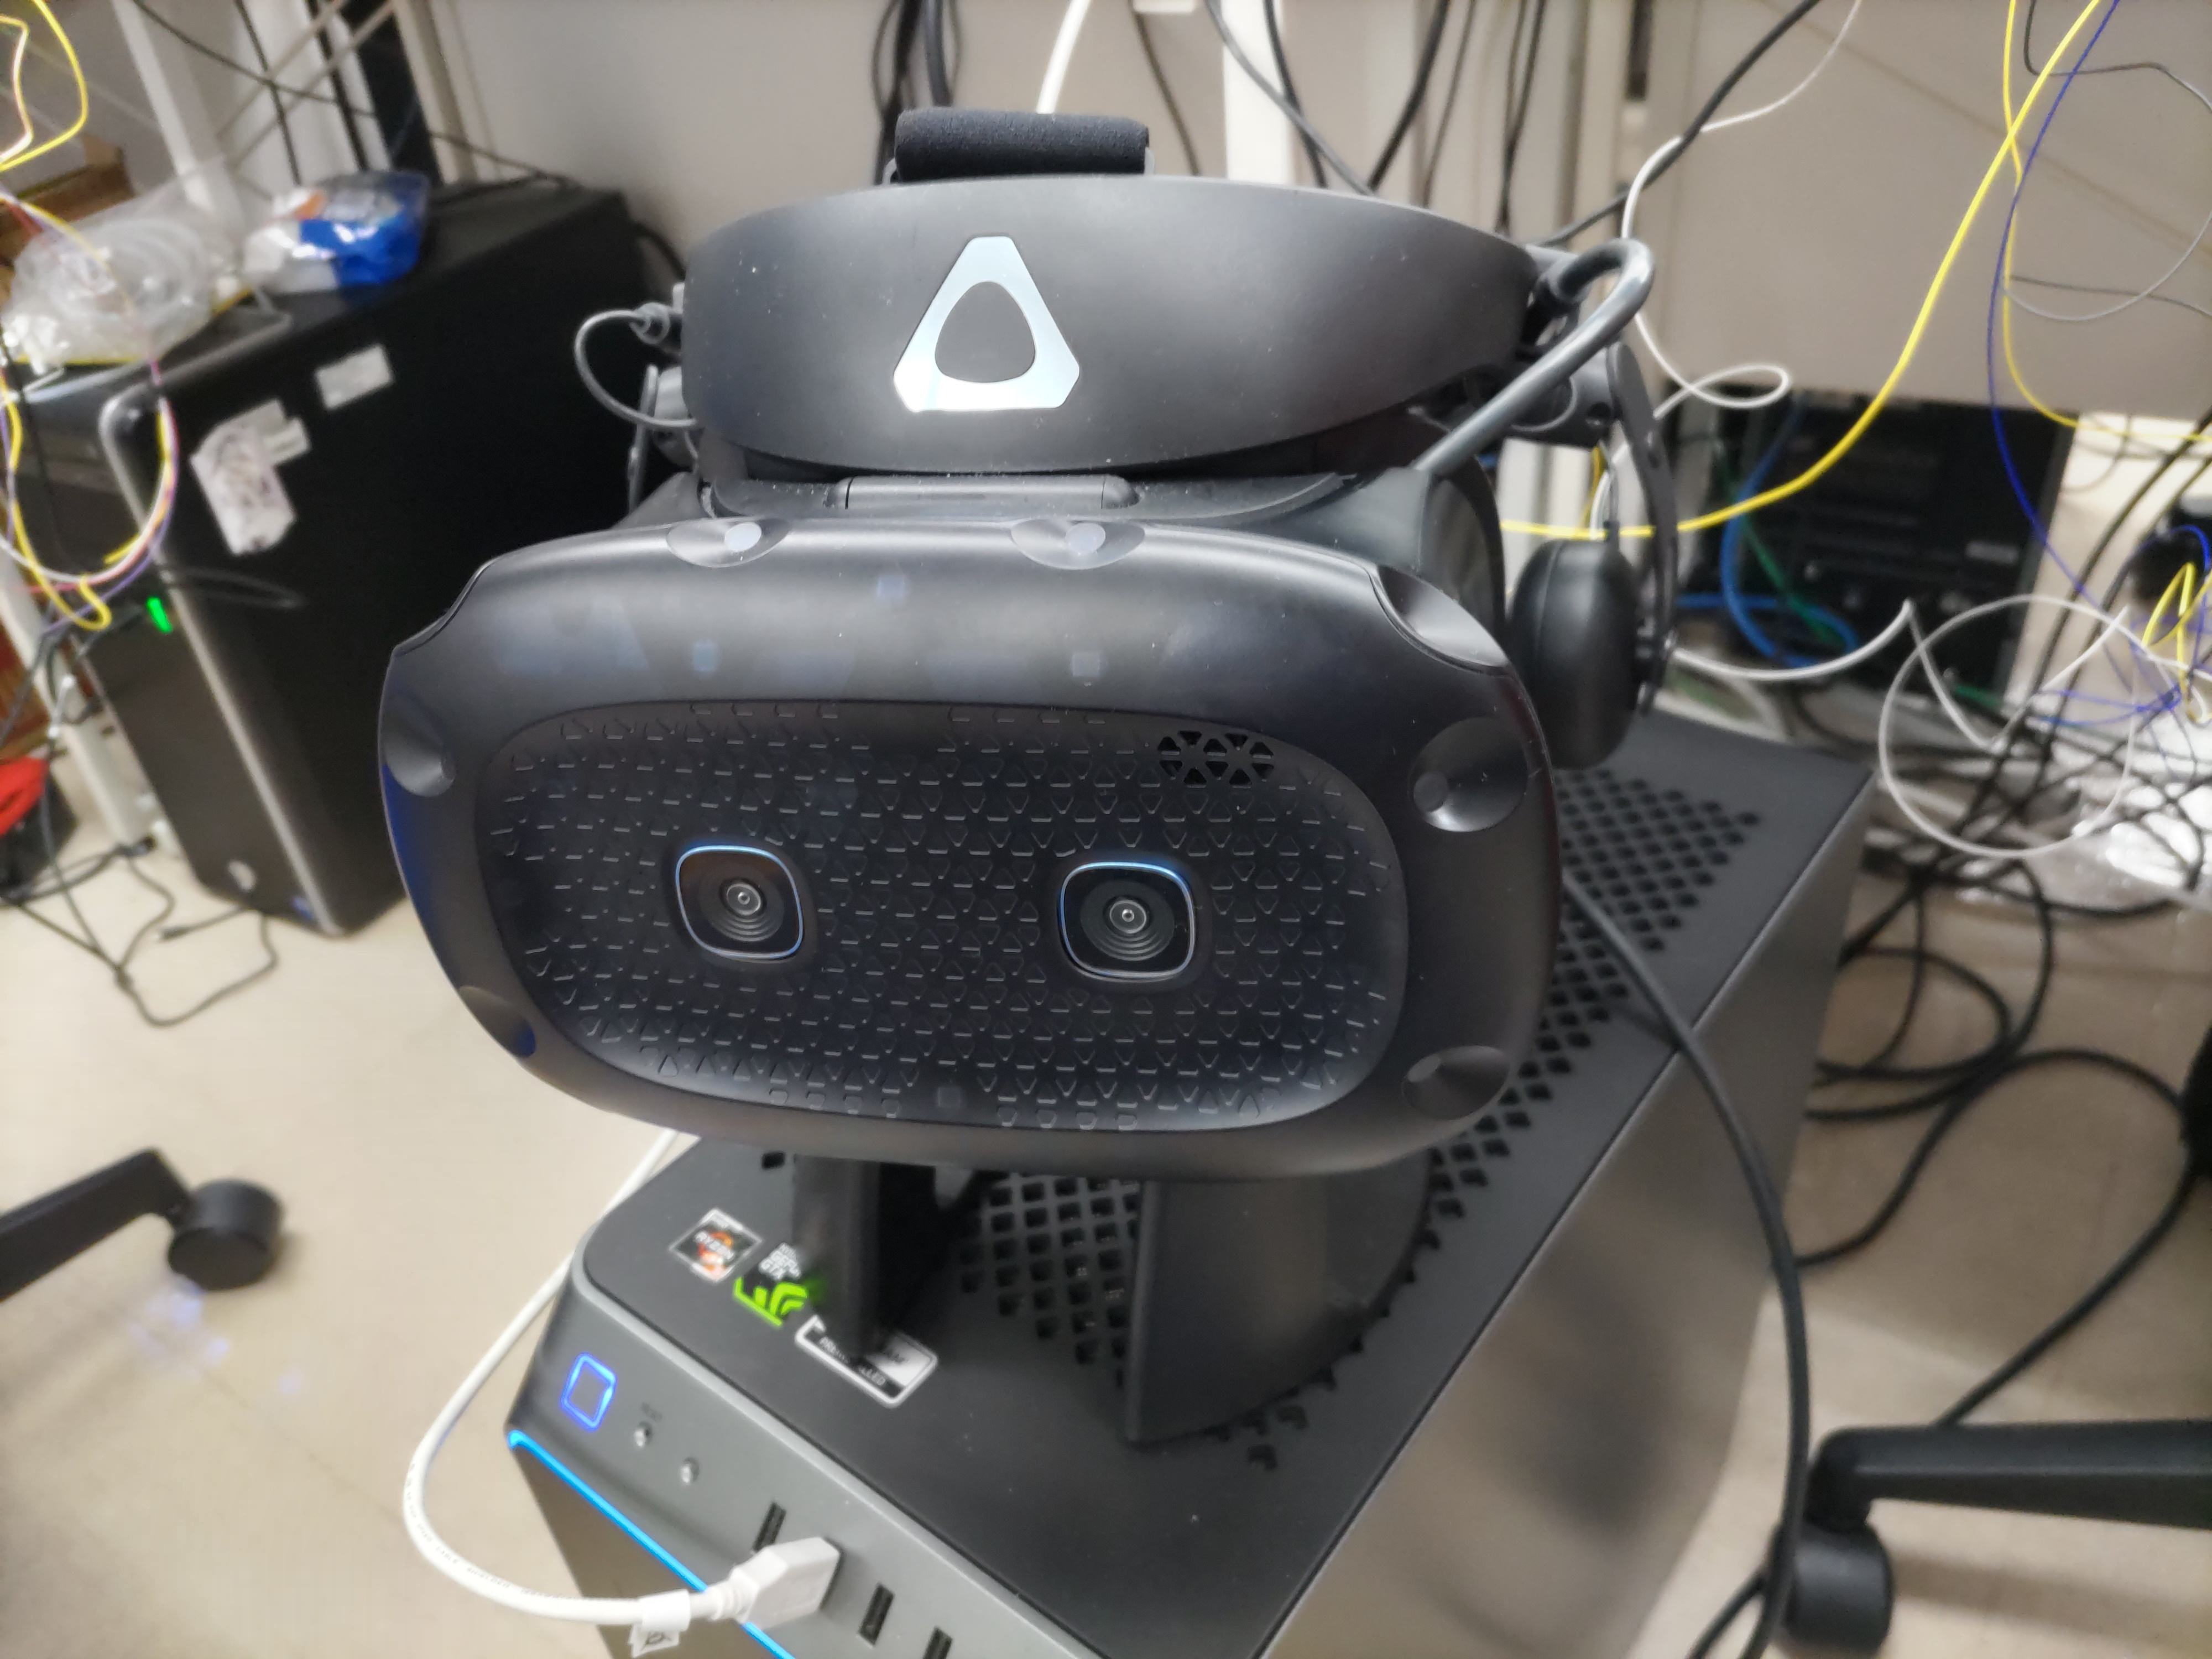
\includegraphics[clip,width=8cm]{./fig/VIVE.png}
\caption{VIVE Cosmos Elite}\label{VIVE}
\end{figure}
本研究で使用したヘッドマウントディスプレイ(以下HMD)をとする)を\figref{VIVE}に示す.
VIVEcosmosEliteはHTCVIVEが開発したヘッドマウントディスプレイの1つである.
VR空間内での座標と方向を取得を取得し,HMD にVR空間を投影する.




\newpage

\section{振動モーター}

\begin{figure}[h]
\centering
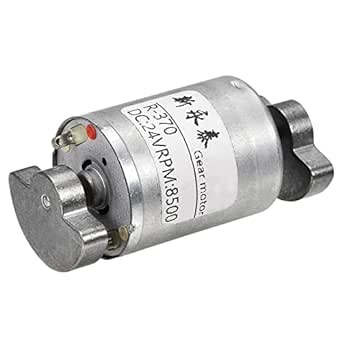
\includegraphics[clip,width=8cm]{./fig/Motor.png}
\caption{振動モーター}\label{motor}
\end{figure}

本研究では,ユーザーに振動刺激を与えるために振動モーターを用いる.使用した振動モーターは\figref{motor}に示す.
振動モーターはユーザーに情報を伝えるほか,触覚フィードバックに使われる.
電流を流すと偏心重錘が回転することにより振動が発生する.


\section{Arduino}
本研究で使用したArduino UNO R3\cite{arduino}(以下Arduinoとする)を\figref{arduino}に示す.
Arduino はArduino S.L.Iによって開発,販売されているマイコンである.
USBを介してPCとの通信が可能であり,本研究ではUnityとのシリアル通信を行っている.

\begin{figure}[h]
\centering
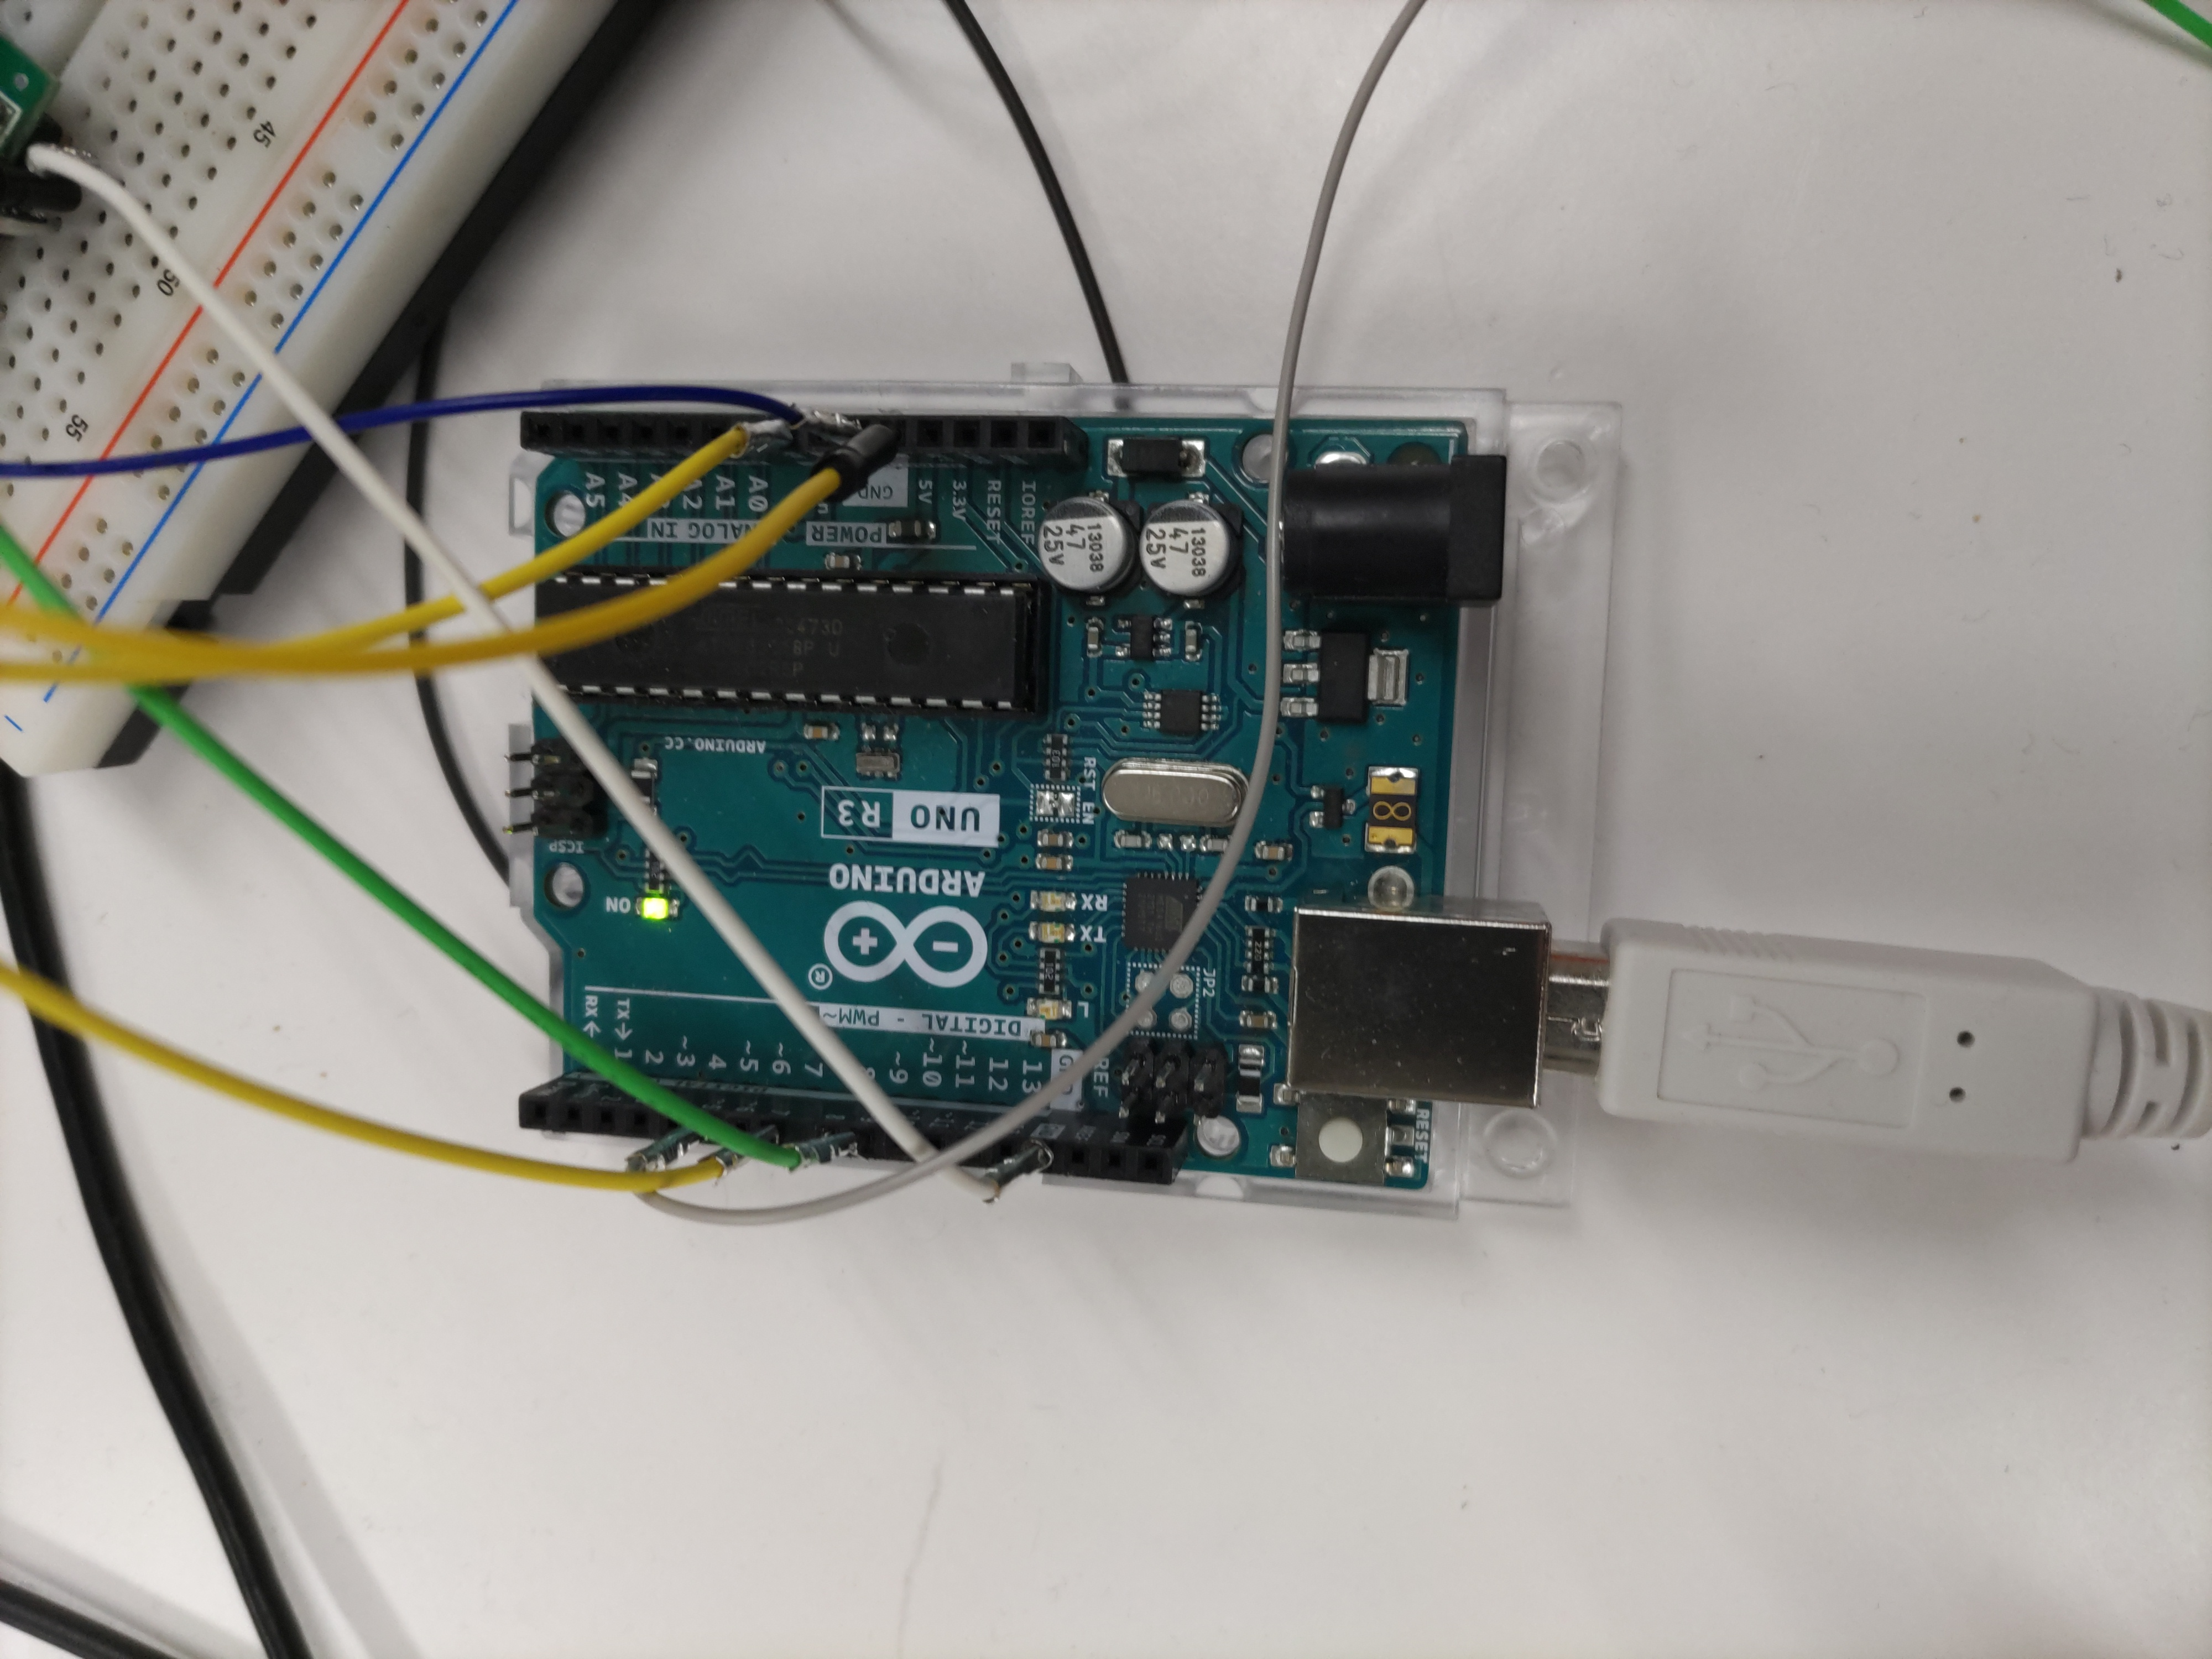
\includegraphics[clip,width=8cm]{./fig/Arduino.png}
\caption{Arduino UNO R3}\label{arduino}
\end{figure}

\newpage

\section{モータードライバ}

\begin{figure}[h]
\centering
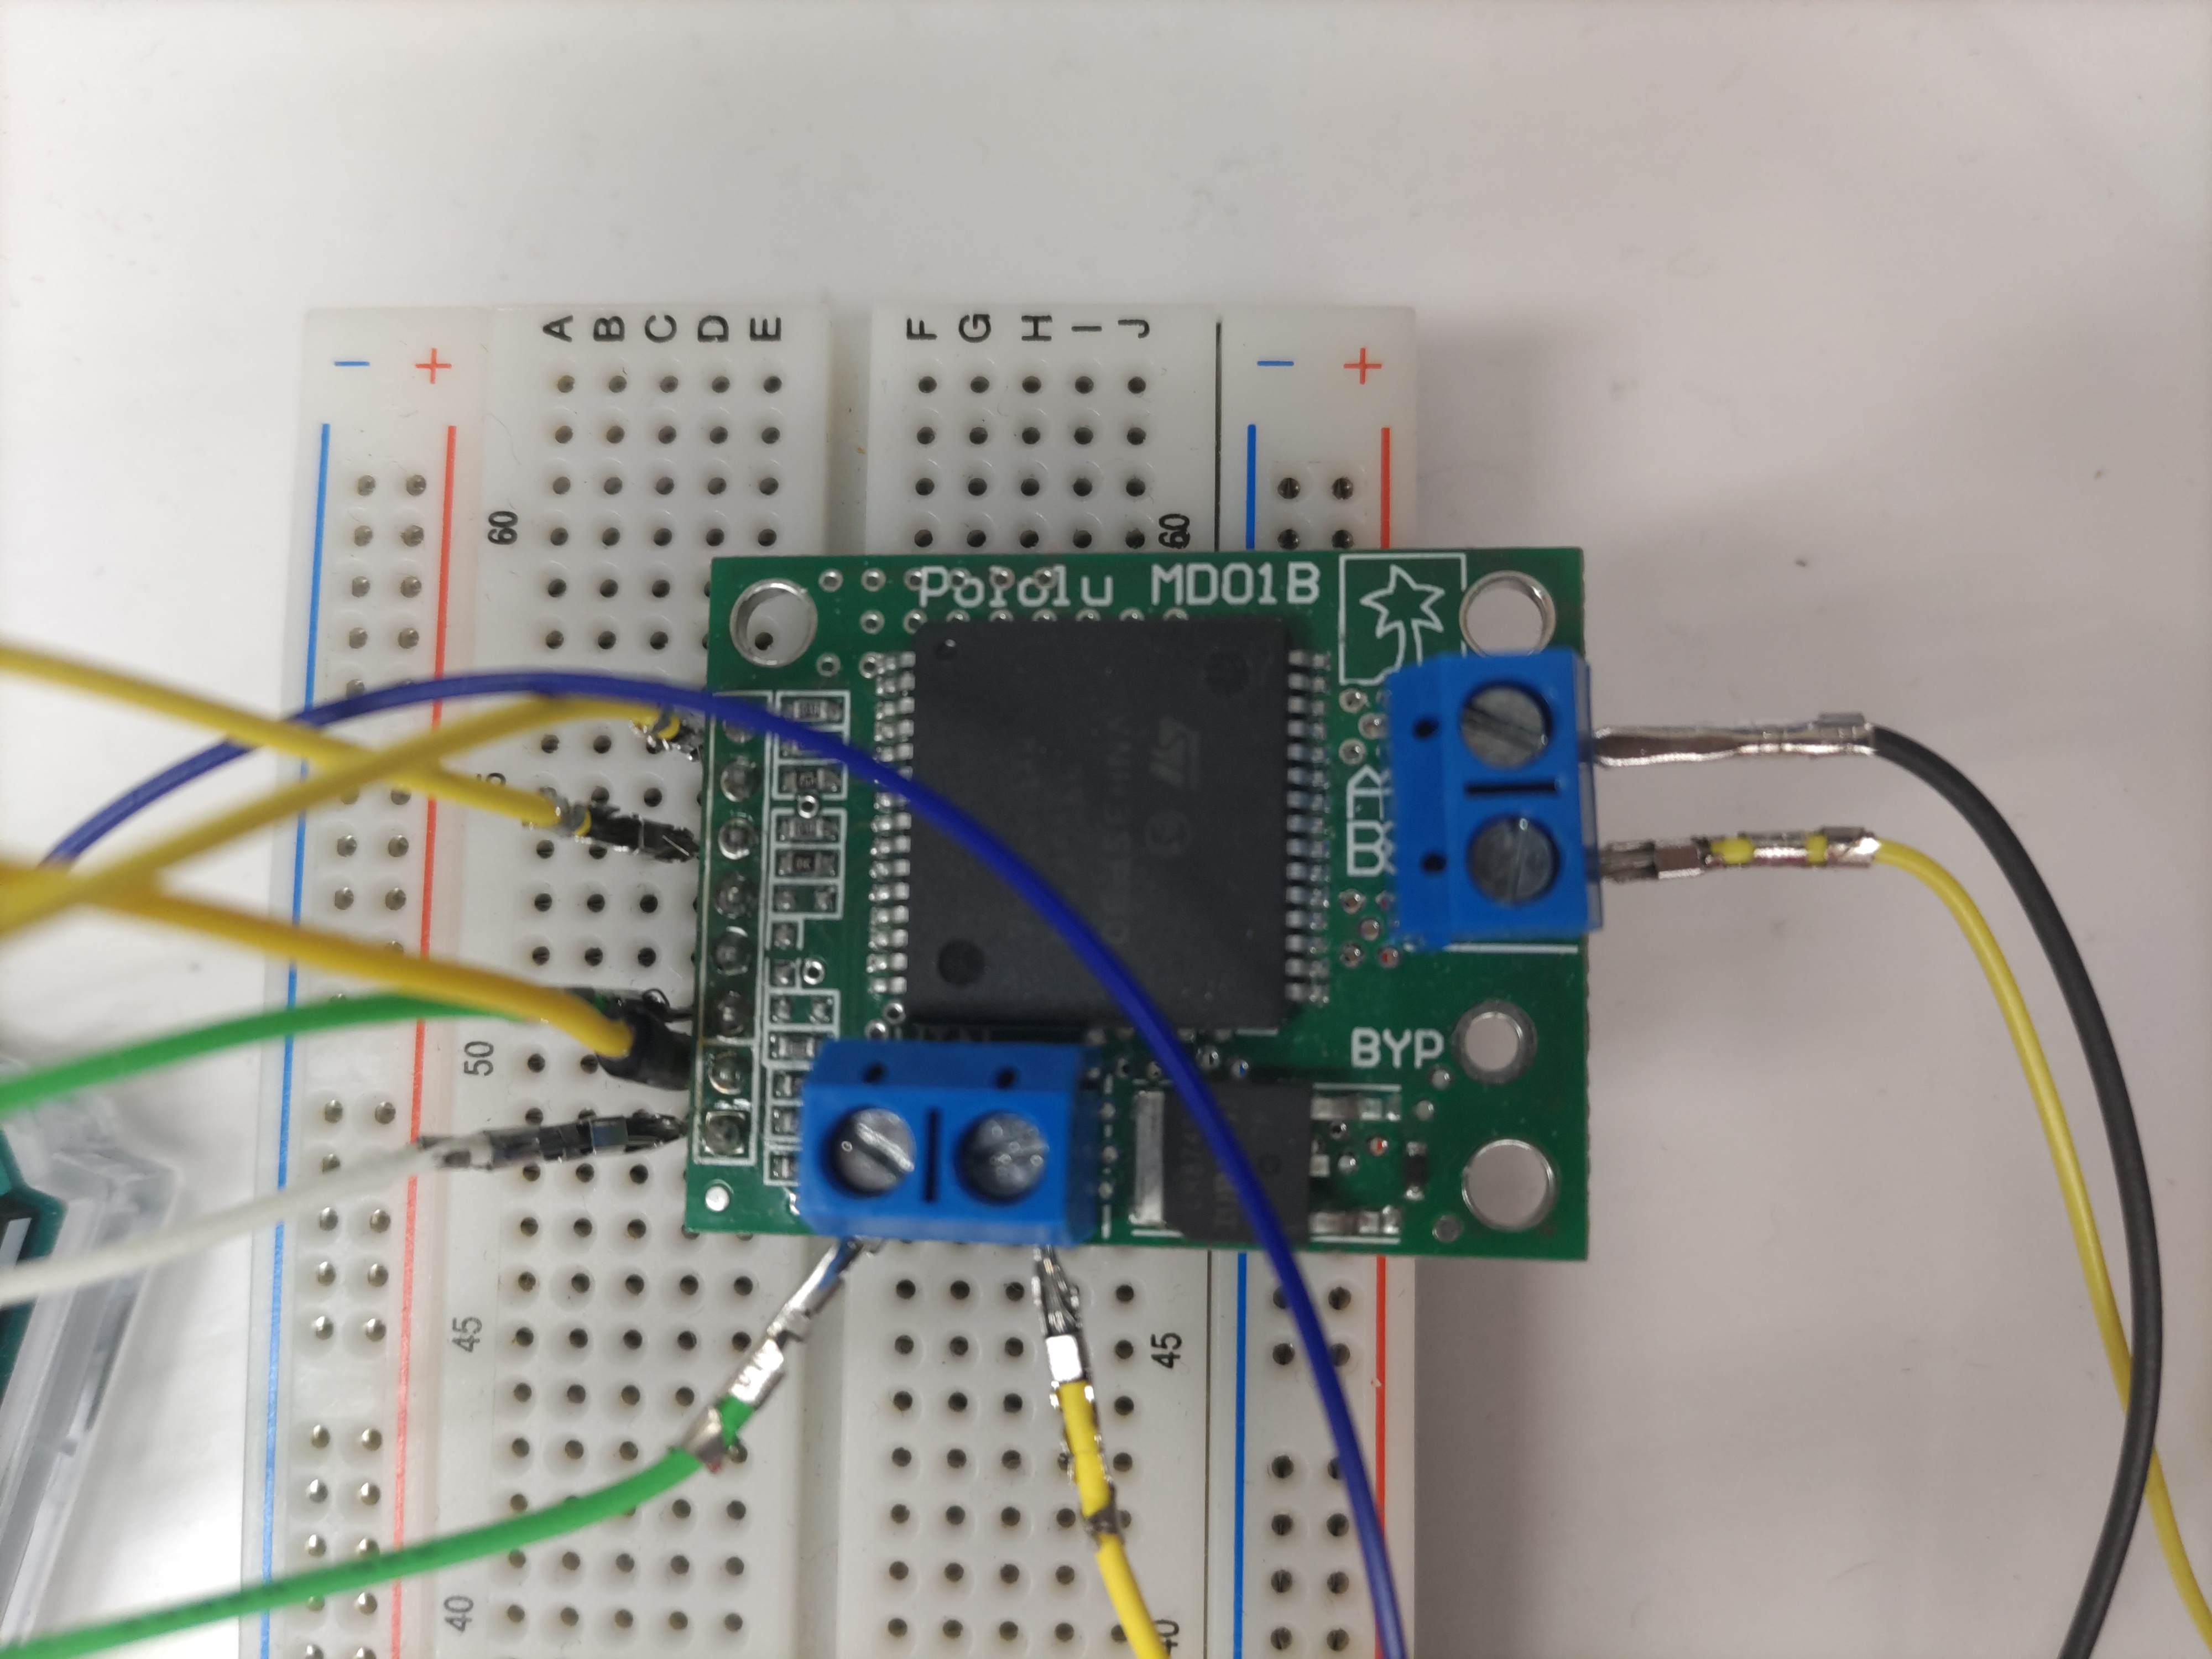
\includegraphics[clip,width=8cm]{./fig/pololuMD01B.png}
\caption{Pololu MD01B}\label{polo}
\end{figure}

\figref{polo}にモータードライバを示す.
モータードライバはマイクロコントローラからの制御信号を受け取り,電動モーターを制御する.
本システムでは,数種類の振動刺激を実装するために使用する.

\newpage

\section{Unity}

\begin{figure}[h]
\centering
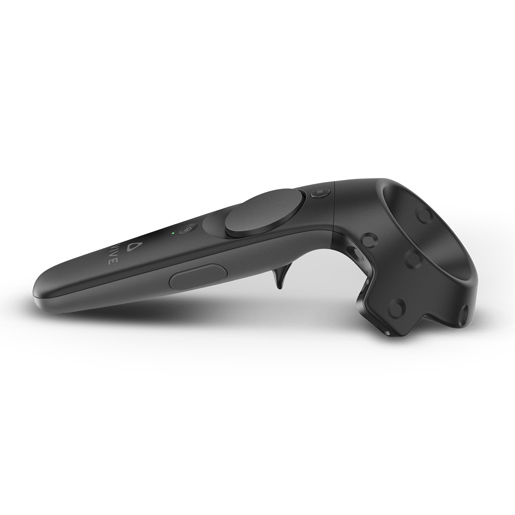
\includegraphics[clip,width=8cm]{./fig/vivecontroller.png}
\caption{Unity上の画面}\label{unity}
\end{figure}

unity\cite{unity}はUnity Technologies社が開発・販売しているゲームエンジンである.ゲーム開発や仮想現実,拡張現実などのアプリケーションを開発するためのゲームエンジンである.プログラミングの初心者からプロの開発者まで利用しやすいため,学習や教育の分野でも利用されている.

unityの開発画面を\figref{unity}に示す.

\section{関連研究}

\subsection{スマートフォンにおける多様な振動フィードバックが被験者の印象に与える影響}
スマートフォンにおける多様な振動フィードバックが被験者の印象に与える影響\cite{smart}の研究を白神らが行った.この研究では振動パターンがユーザーに与える印象に焦点を当て,約250通りの振動パターンからユーザーがどのような印象を持ったのかを調査したものである。


しかし,この研究は,スマホという掌の上での振動でしかなく,さらに大きな物体での振動についての調査は行っていない.
また,実際に存在しているものに関する振動についての調査なので,魔法という非現実的なものに対する振動については明かされていない.






%%%%%%%%%%%%%%%%%%%%%%%%%%%%%%%%%%%%%%%%%%%%%%%%%%%%%%%%%%%%%%%%%%%%%%%
\begin{comment}
  \begin{textblock}{6.5}(1, 18)
    \noindent
    【16,18】図番号は章ごとの通し番号で抜けがない
  \end{textblock}
  
  \begin{textblock}{7}(13, 22)
    ←本文で説明がない図は載せない
  \end{textblock}
\end{comment}
%%%%%%%%%%%%%%%%%%%%%%%%%%%%%%%%%%%%%%%%%%%%%%%%%%%%%%%%%%%%%%%%%%%%%%%     % 第2章
\chapter{VRゲーム上で振動刺激のある魔法体験における没入感体験向上システム}
本研究では、VRを用いてユーザーの魔法体験における没入感を向上させるシステムを提案、開発し、視覚エフェクトと振動刺激の組み合わせによってユーザーの没入感にどのような影響を与えるのかを調査する.





%%%%%%%%%%%%%%%%%%%%%%%%%%%%%%%%%%%%%%%%%%%%%%%%%%%%%%%%%%%%%%%%%%%%%%%
\begin{comment}
    \begin{textblock}{4.5}(1, 21.5)
        \noindent
        【16,18】表番号は章ごとの通し番号で抜けがない
    \end{textblock}
    \begin{textblock}{5}(14.5, 13)
        ←表のキャプションは上
    \end{textblock}
\end{comment}
%%%%%%%%%%%%%%%%%%%%%%%%%%%%%%%%%%%%%%%%%%%%%%%%%%%%%%%%%%%%%%%%%%%%%%%
\section{システム概要}
\figref{allsystem}に本システムの概要を示す.
\begin{figure}[h]
\centering
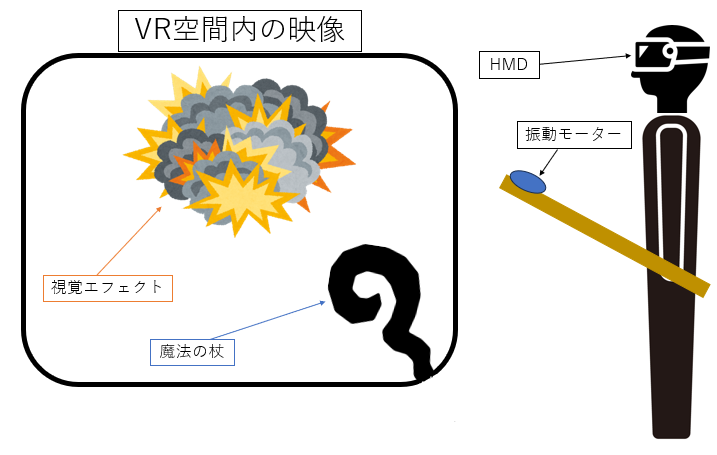
\includegraphics[clip,width=9cm]{./fig/allsystem.png}
\caption{システム概要}\label{allsystem}
\end{figure}

本研究では被験者が右手にコントローラーを持った状態でヘッドマウントディスプレイを装着する.
被験者がコントローラに装着されている押しボタンを押すことで視覚エフェクトと振動刺激が被験者に提示される.
提示する視覚エフェクトと振動刺激は実験者がPCから決定する.

\section{振動提示手法}
本研究では,振動提示の方法として振動モーターを使用した.
振動子をガムテープで木の角材に固定する.
被験者がこの角材を把持することによって角材を媒体とし被験者の手に伝わることで振動を提示できるようにした.


\newpage

\section{魔法エフェクトの選定}
実装する視覚エフェクトは,形状が異なりユーザーに与えられる振動刺激が異なると思われる3種類の視覚エフェクトを選定した.

以下に選定した3種類の視覚エフェクトを示す.

incenerationは火が燃え続けるエフェクトである.
main-beamは最初に大きな爆発があり,その後爆発の余韻が残るエフェクトである.
ring-fireは初めにエネルギーをためるフェーズがあり,その後ためたエネルギーを一気に解放するエフェクトである.

\begin{figure}[h]
\centering
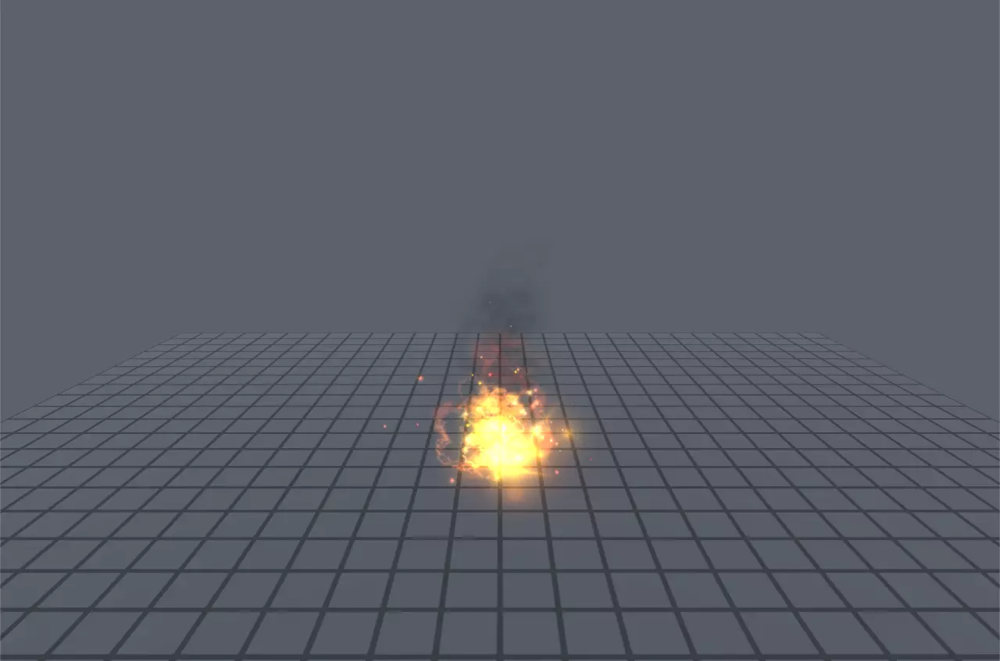
\includegraphics[clip,width=6.5cm]{./fig/firefire.png}
\caption{inceneration}\label{fire}
\end{figure}

\begin{figure}[h]
\centering
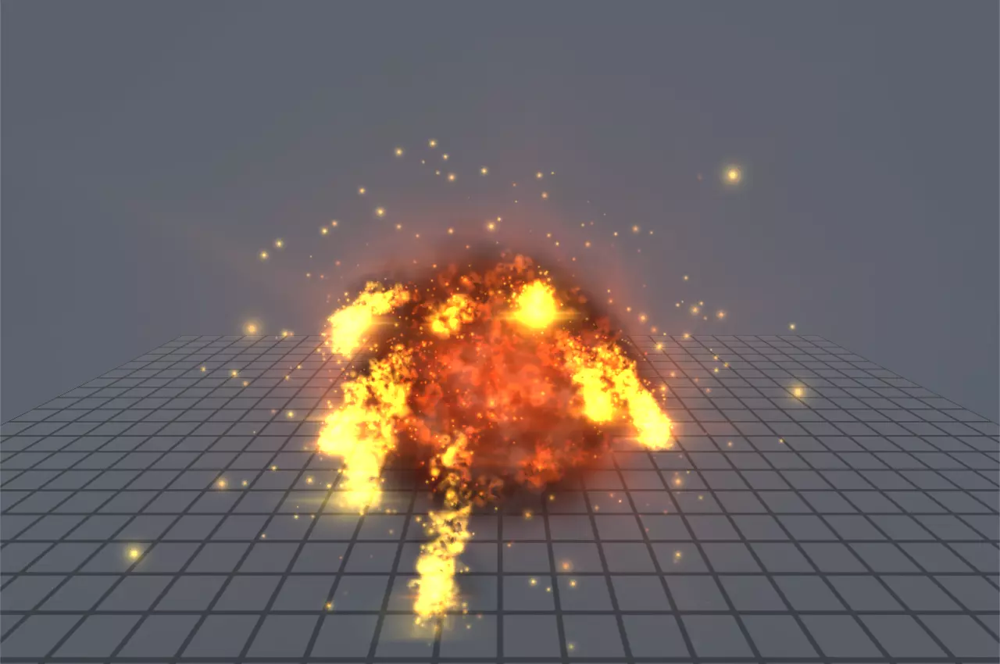
\includegraphics[clip,width=6.5cm]{./fig/explosion.png}
\caption{main-beam}\label{explosion}
\end{figure}

\begin{figure}[h]
\centering
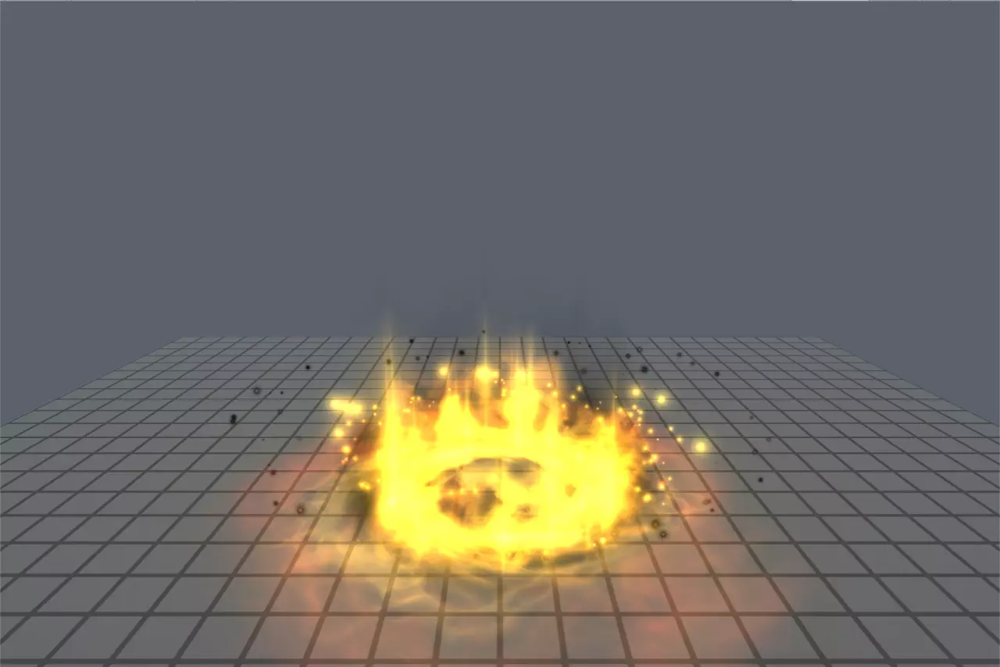
\includegraphics[clip,width=6.5cm]{./fig/ringfire.png}
\caption{ring-fire}\label{ringfire}
\end{figure}


\newpage
\subsection{振動パターンの選定}
以下に選定した4種類の振動パターンを示す.振動強度が一定,弱~強,強~弱,矩形波の4種類である.
それぞれ順にパターン1,パターン2,パターン3,パターン4とする.

矩形波とは,波形を時間領域で見たときに方形状を持つ波のことである.
振動が一定間隔で高低2つの一定値を繰り返す.
本研究では低い振動を振動させないようにしている.
そのため一定期間で振動子が動いたり止まったりを繰り返す挙動をとる.

\begin{table}[H]
    \caption{\label{tab;sindou}振動パターンと内容}
    \centering
    \begin{tabular}{l|l}
    \hline
    \hline
    パターン1 & 一定\\
    パターン2 & 弱→強\\
    パターン3 & 強→弱\\
    パターン4 & 矩形波\\
    \hline
    \end{tabular}
\end{table}


\begin{figure}[h]
\centering
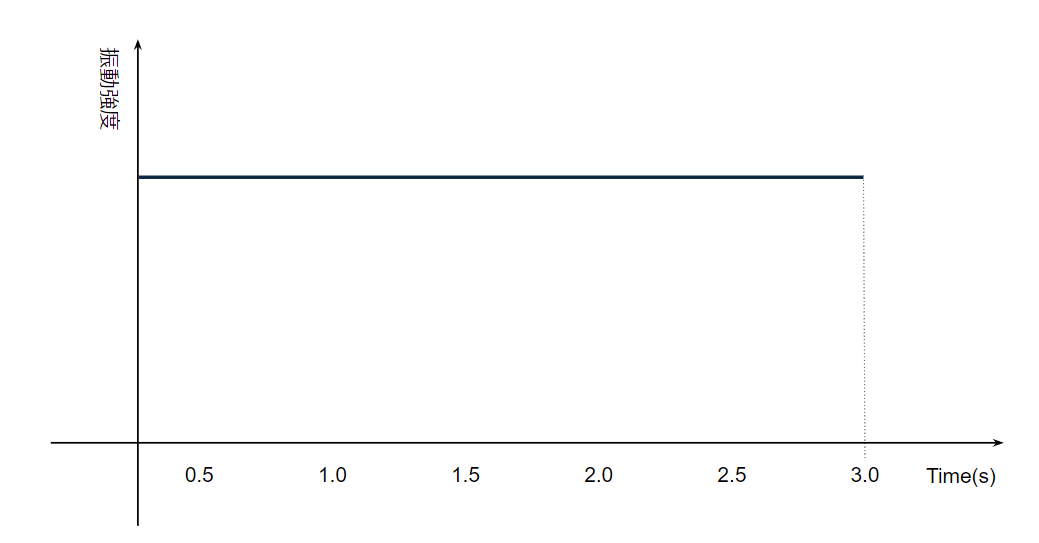
\includegraphics[clip,width=10cm]{./fig/patarn1.png}
\caption{パターン1}\label{patarn1}
\end{figure}

\begin{figure}[h]
\centering
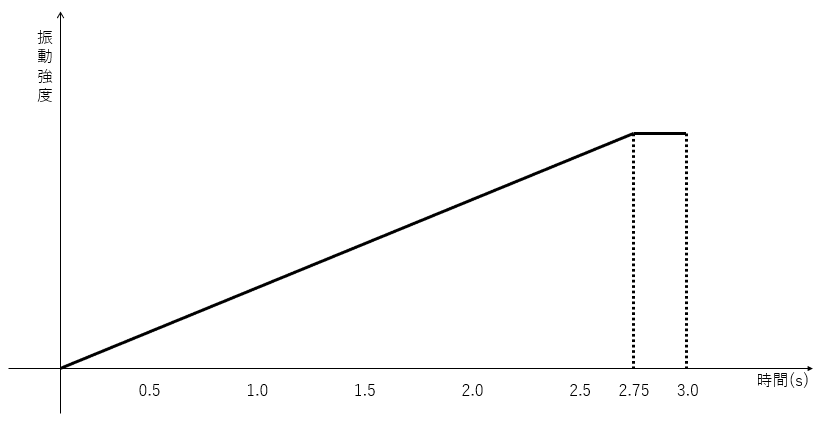
\includegraphics[clip,width=10cm]{./fig/patarn2.png}
\caption{パターン2}\label{patarn2}
\end{figure}

\begin{figure}[h]
\centering
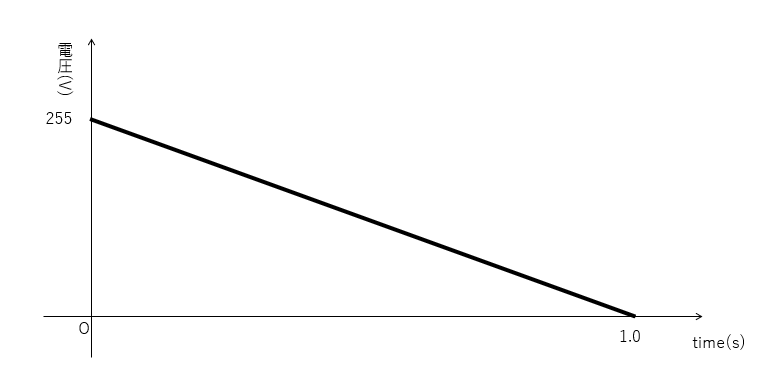
\includegraphics[clip,width=10cm]{./fig/patarn3.png}
\caption{パターン3}\label{patarn3}
\end{figure}

\begin{figure}[h]
\centering
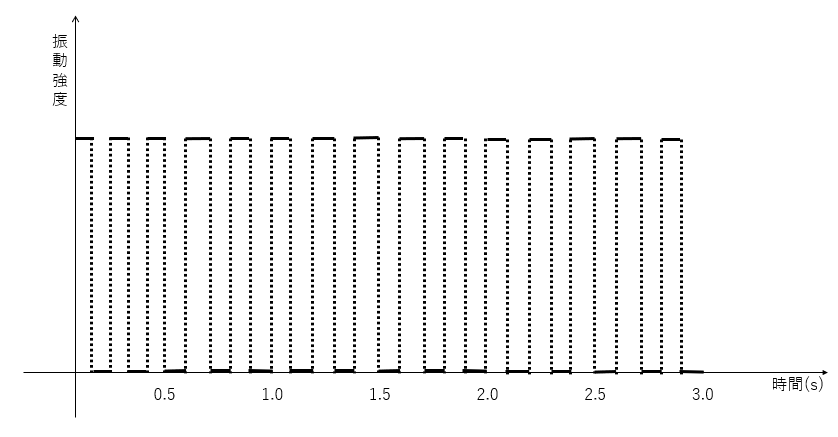
\includegraphics[clip,width=10cm]{./fig/patarn4.png}
\caption{パターン4}\label{patarn4}
\end{figure}


    % 第3章
\chapter{実装}
本章では,本研究の実装環境をハードウェアとソフトウェアに分けて説明する.

\section{ハードウェアシステム構成}
本システムの構成を\figref{sys}に示す.本システムは主にHMD,VIVEトラッカー,PC,角材,振動モーター、押しボタンで構成される.被験者はHMDを装着した状態で右手にコントローラーを持つ.ベースステーションでコントローラ―に取り付けられたVIVEトラッカーを読みとりPCに情報を送信する.その情報をもとに仮想空間上に魔法の杖を表示しHMDに描画する.

\begin{figure}[h]
\centering
\includegraphics[clip,width=10cm]{./fig/systemP.png}
\caption{システム構成}\label{sys}
\end{figure}

\newpage

\subsection{コントローラー}
上記の構成の中で角材,押しボタン,VIVEトラッカーでコントローラーを構成している.押しボタンを押すことでArduinoに信号を送る.Arduinoが信号を受信するとモータードライバに信号を送り振動モーターを回転させ,コントローラ―を振動させる.
\figref{controller}に本システムのコントローラーを示す.

\begin{figure}[h]
\centering
\includegraphics[clip,width=10cm]{./fig/controller.png}
\caption{コントローラー}\label{controller}
\end{figure}





%----------------------------------------------------------------------------------------------

\subsection{ソフトウェア}
本研究ではUnityを用いてシステムを開発した.
に使用したOSを\tabref{tab;software}に示す.

\begin{table}[H]
    \caption{\label{tab;software}ソフトウェア実装環境}
    \centering
    \begin{tabular}{l|l}
    \hline
    \hline
    OS & Windows 11\\
    開発言語 & C\#\\
    ゲームエンジン & Unity(2021.1.15f1)\\
    \hline
    \end{tabular}
\end{table}

\subsection{視覚エフェクトと振動刺激提示の連動}
前述したコントローラーに装着されている押しボタンを押すとArduinoに信号が送られ,信号を受け取ったArduinoからモータードライバとunityに信号を送信することで視覚エフェクトと振動刺激の提示を連動させている.

\subsection{Unity}
\ref{virtualworld}に開発した仮想世界を示す.仮想世界には魔法の杖と足場がある.魔法の杖は現実空間のコントローラーの動きと同期している.コントローラーのボタンを押すと仮想空間上に視覚エフェクトが表示される.そのときArduinoとシリアル通信を行い振動モーターを回転させる.

\begin{figure}[h]
\centering
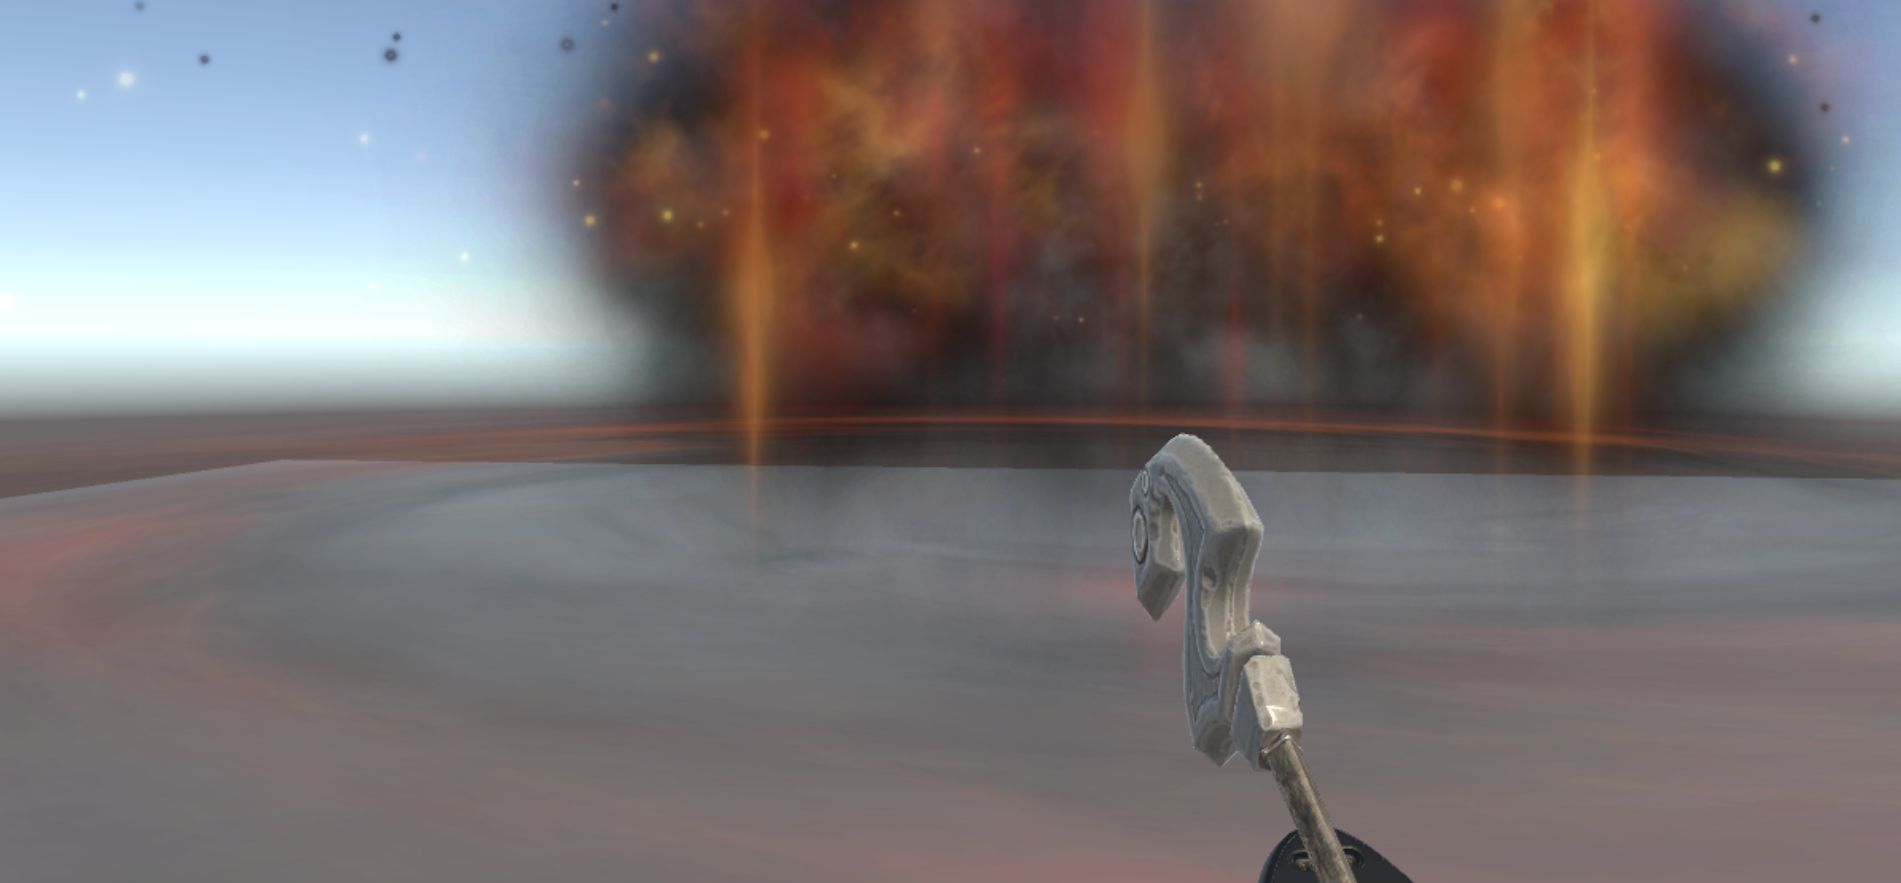
\includegraphics[clip,width=10cm]{fig/unity.png}
\caption{仮想空間}\label{virtualworld}
\end{figure}







%%%%%%%%%%%%%%%%%%%%%%%%%%%%%%%%%%%%%%%%%%%%%%%%%%%%%%%%%%%%%%%%%%%%%%%
\begin{comment}
    \begin{textblock}{2}(1, 16.5)
        空行→
    \end{textblock}
    
    \begin{textblock}{2}(1, 18.5)
        字下げ→
    \end{textblock}
        
    \begin{textblock}{2}(1, 20.5)
        空行→
    \end{textblock}
    
    \begin{textblock}{11}(9, 20.5)
        ←読点までが元の文なので文献番号はその後につける
    \end{textblock}
    
    \begin{textblock}{7}(14, 26.5)
        ↑同じく読点までが元の文なので
    
        "」"と文献番号はその後につける
    \end{textblock}
\end{comment}
%%%%%%%%%%%%%%%%%%%%%%%%%%%%%%%%%%%%%%%%%%%%%%%%%%%%%%%%%%%%%%%%%%%%%%%    




%%%%%%%%%%%%%%%%%%%%%%%%%%%%%%%%%%%%%%%%%%%%%%%%%%%%%%%%%%%%%%%%%%%%%%%
\begin{comment}
    \begin{textblock}{11}(9, 7.5)
        \noindent
        ↑間接引用では節末・文末の句読点の「前」に文献番号をつける
    \end{textblock}
\end{comment}
%%%%%%%%%%%%%%%%%%%%%%%%%%%%%%%%%%%%%%%%%%%%%%%%%%%%%%%%%%%%%%%%%%%%%%%




   % 第4章
\chapter{実験}
本章では,提案する視覚エフェクトと振動刺激の提示手法を用いた評価実験を行った.本章では実験内容及びその結果を示す.

評価実験では,VR上に魔法の杖を表示しそこから特定の形状の魔法を放つ.
それに伴い,ユーザーに対しさまざまな振動刺激を与える.
これにより魔法の形状に対してどのような振動刺激をユーザーに与えることで,ユーザーの魔法体験感を高めることができるのかを調査する.

\section{実験方法}
本章では作成したシステムを用いた評価実験を行った.
22歳$\sim$24歳の男性8名に対して実験を実施した.

\subsection{実験手順}
本実験の手順を以下に示す.
手順の2$\sim$4の工程をinceneration,ring-fire,main-beamの順番にそれぞれ繰り返す.
被験者は振動を体験してもらった後,アンケートに回答してもらうので振動パターンを覚えておく必要がある.
その旨を実験説明の段階で被験者に伝える.

\begin{enumerate}
    \item 実験説明
    \item 実験前アンケート
    \item 実験
    \item 実験後アンケート
\end{enumerate}

\newpage
\section{評価実験}
\subsection{実験前アンケート}
実験を実施する前にアンケートを行う.

まず,被験者に実験で使用する視覚エフェクトの動画を見せる.
次に視覚エフェクトを時系列順に6分割し並べた画像を被験者に見せる.
それぞれ振動強度がどのように変化しそうであるか,被験者のイメージを手書きでグラフに書いてもらった.
振動強度のグラフを\figref{ank}に示す.

ユーザーが視覚エフェクトに対してどのような振動刺激が与えられるとイメージしているのかを調査する.

\begin{figure}[h]
\centering
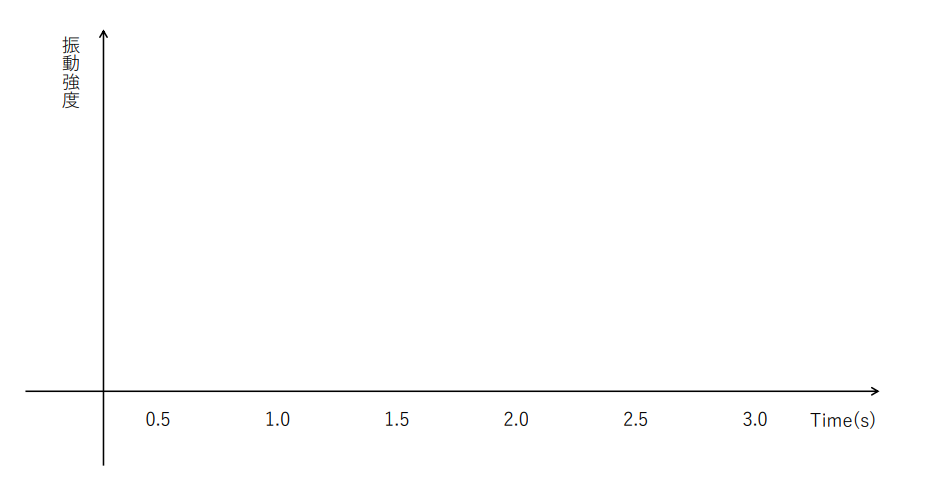
\includegraphics[clip,width=10cm]{./fig/ank.png}
\caption{振動強度のイメージ}\label{ank}
\end{figure}

\subsection{実験}
被験者はHMDを装着し右手にコントローラーを持つ.実験の様子を\figref{jikken}に示す.
提示する視覚エフェクトと振動パターンを実験者が選択する.この時被験者に選択したエフェクトを伝えておく.
視覚エフェクトに対して4パターンの振動刺激を提示した後アンケートを実施する.これを視覚エフェクトの種類ごとに繰り返す.
実験の被験者の視界を\figref{first}に示す.

\begin{figure}[h]
\centering
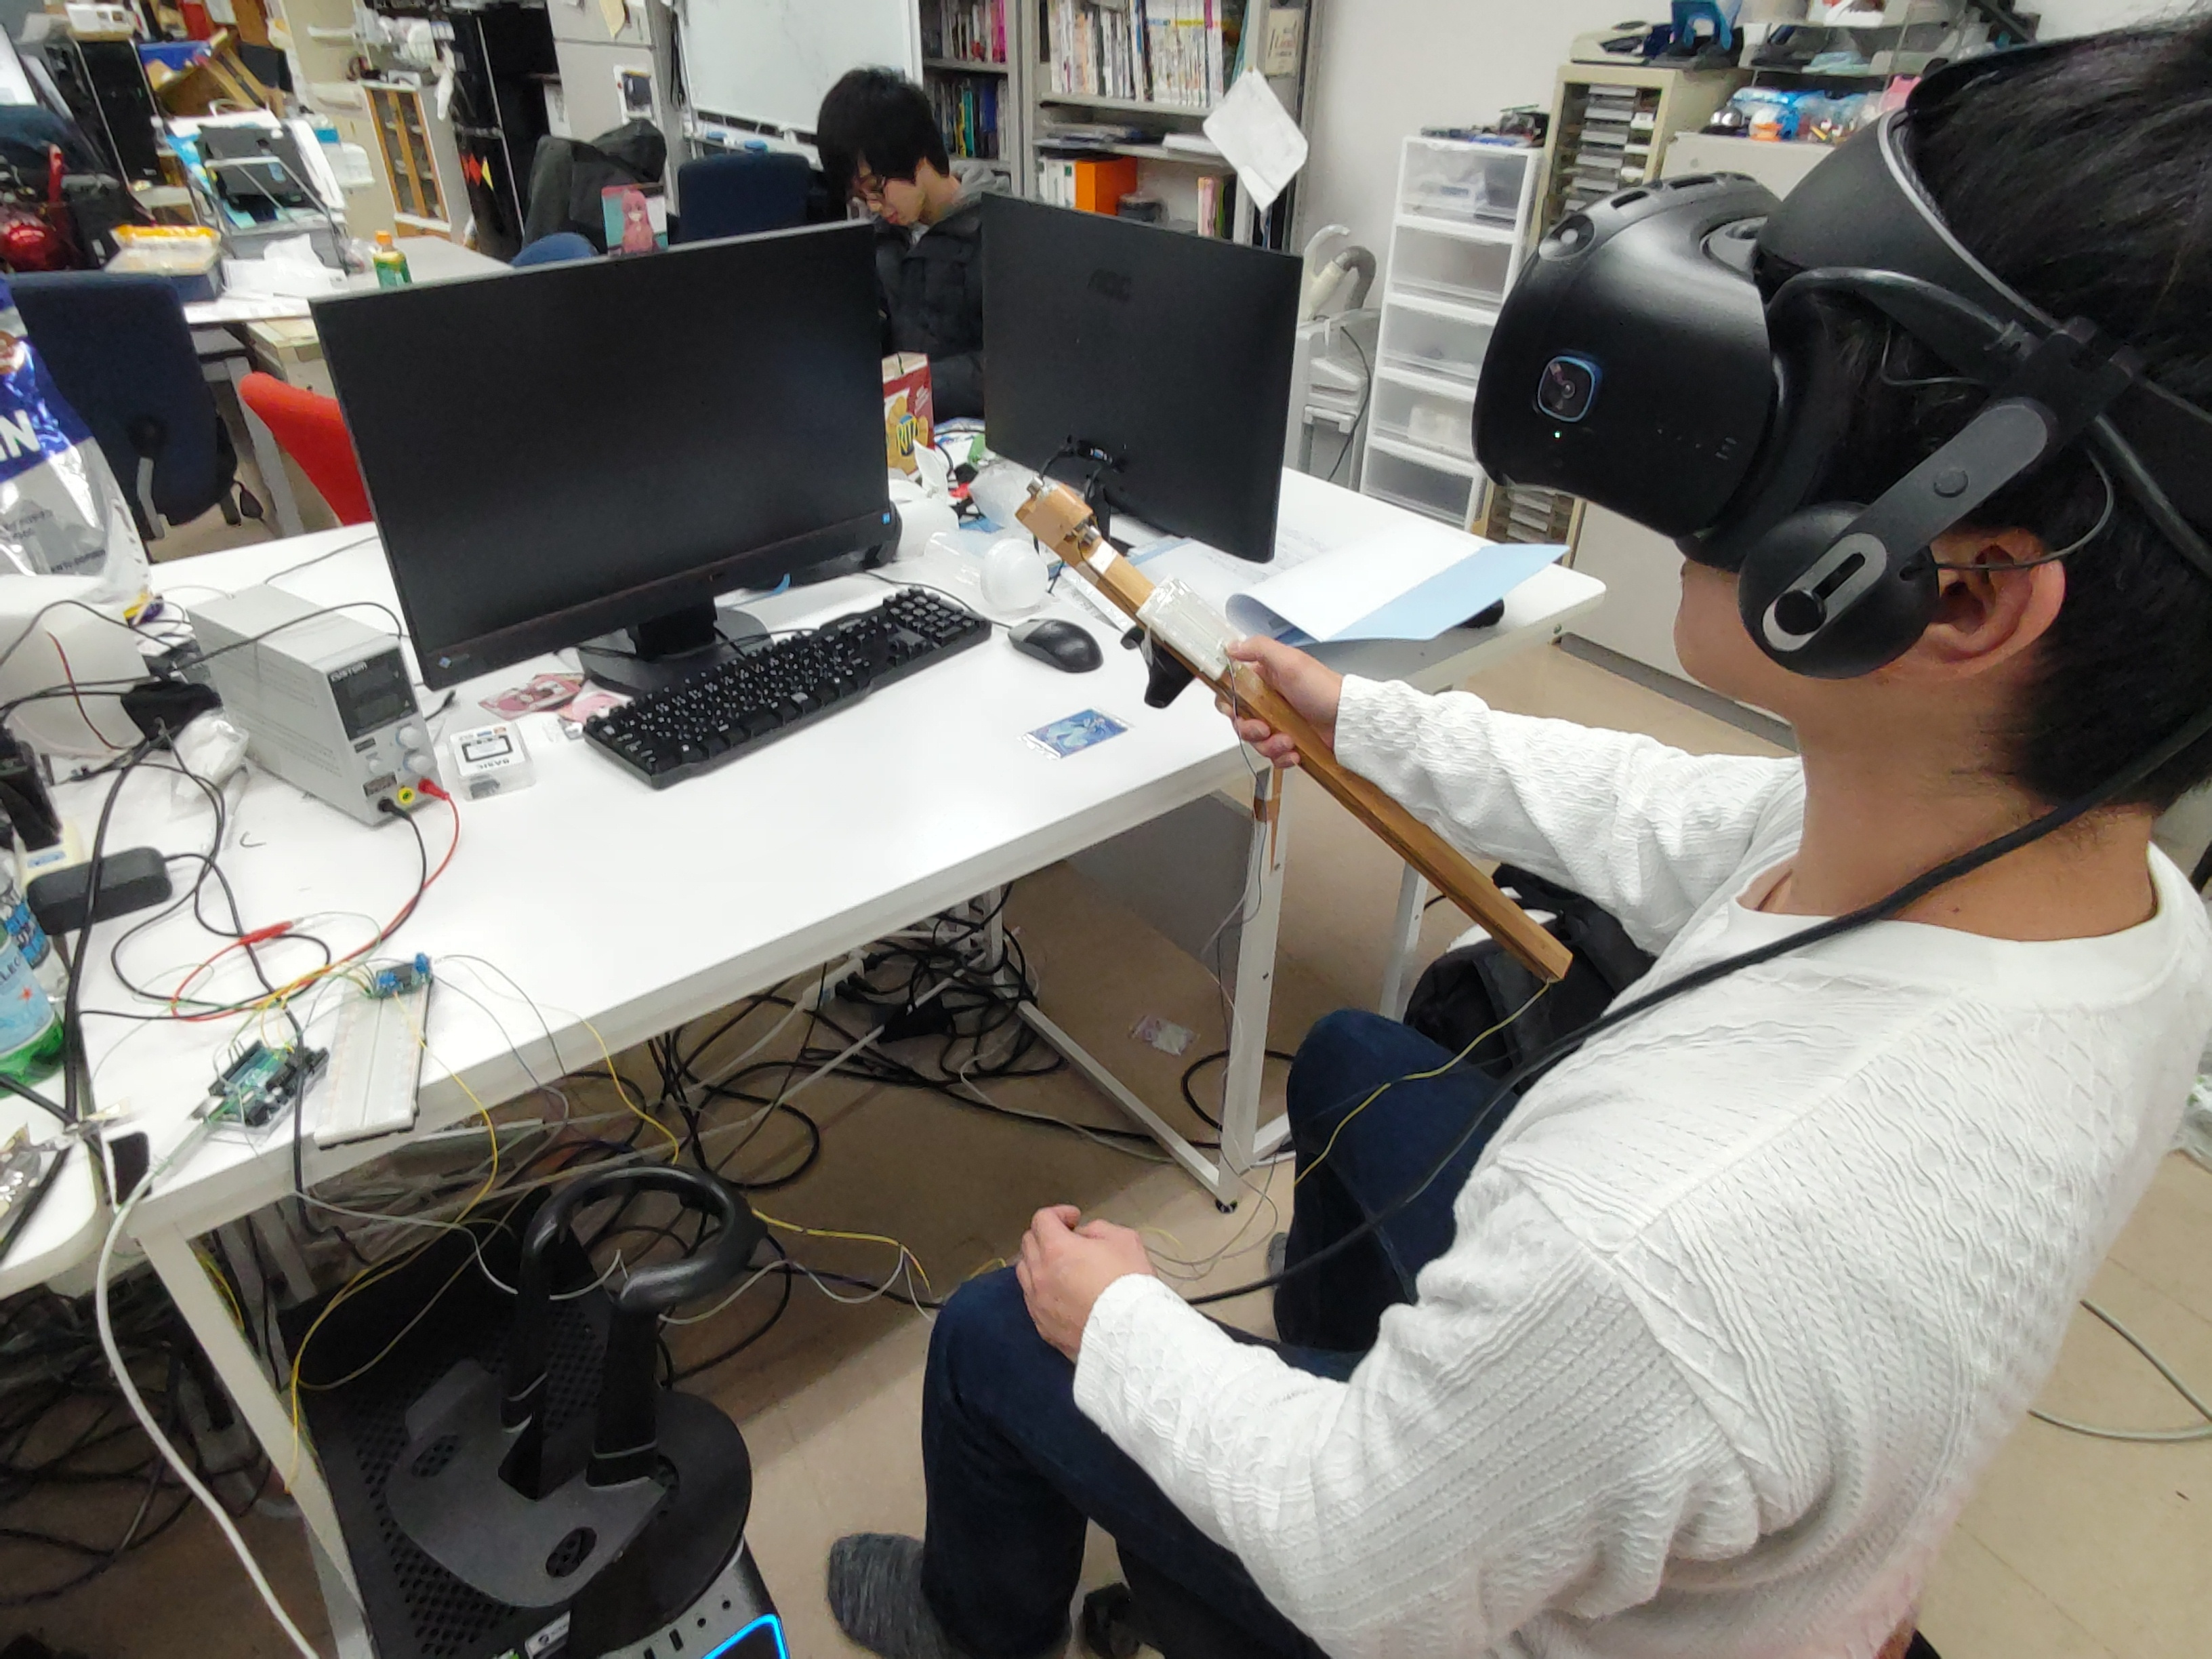
\includegraphics[clip,width=10cm]{./fig/jikken.JPG}
\caption{実験の様子}\label{jikken}
\end{figure}


\begin{figure}[h]
\centering
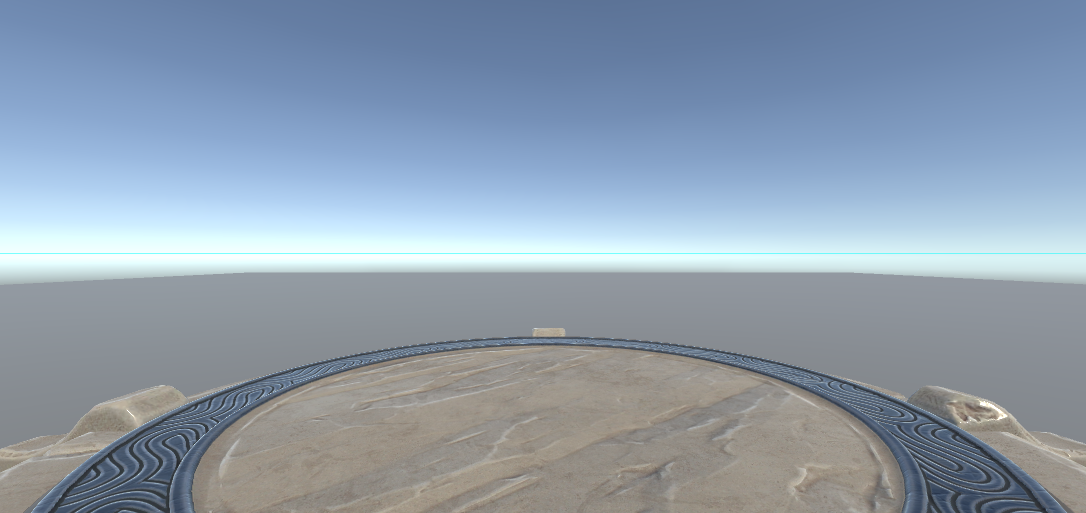
\includegraphics[clip,width=10cm]{./fig/unity_first.png}
\caption{被験者の視界}\label{first}
\end{figure}

実験終了後にアンケートを行う.実験終了後アンケートでは視覚エフェクトに対しての振動刺激の一致度を5段階で評価してもらった.
システム使用中の没入感やその他気になったことや感想は自由記入形式で回答してもらった.

\newpage

\section{結果と考察}
\subsection{実験前アンケート結果}
以下に実験前アンケートの結果を示す.
\figref{inceA}にincenerationについてのアンケート結果を示す.
被験者ほぼ全員がincenerationの振動について,一定であると回答した.
振動パターン1に近い結果となった.
\begin{figure}[h]
\centering
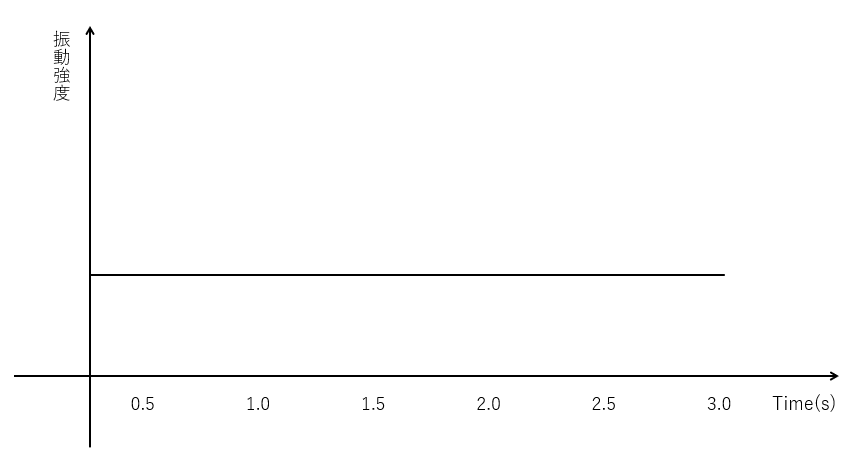
\includegraphics[clip,width=10cm]{fig/incenerationAve.png}
\caption{アンケート結果(inceneration)}\label{inceA}
\end{figure}


\figref{ringA}にring-fireについてのアンケート結果を示す.
2枚目までは小さい振動が続き,3枚目で大きな振動になり,残りは余韻といったイメージであることが分かる.
振動パターン2に近い結果となった.
\begin{figure}[h]
\centering
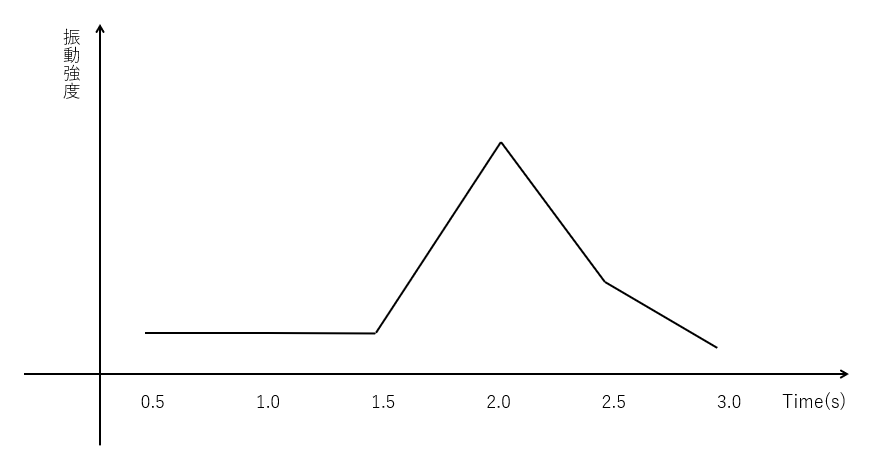
\includegraphics[clip,width=10cm]{fig/ringfireAve.png}
\caption{アンケート結果(ring-fire)}\label{ringA}
\end{figure}



\figref{mainA}にmain-beamについてのアンケート結果を示す.
ring-fireと比較して初めから強い振動があり,残りは余韻といったイメージであることが分かる.
振動パターン3に近い結果となった.
\begin{figure}[h]
\centering
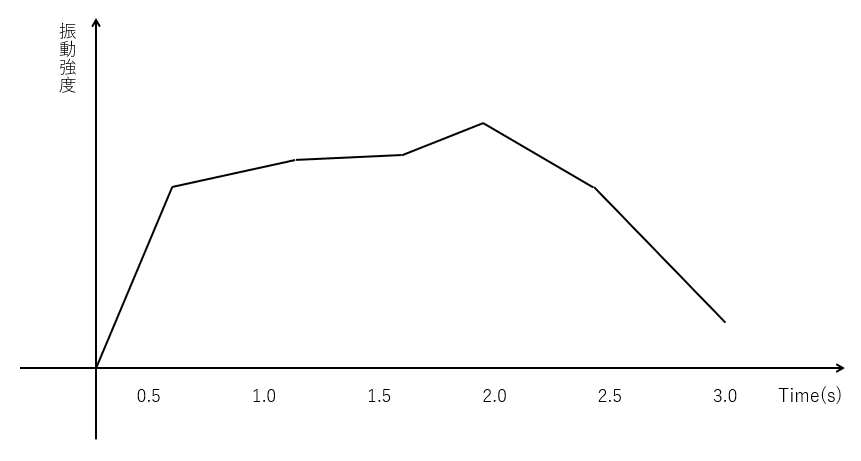
\includegraphics[clip,width=10cm]{fig/mainbeamAve.png}
\caption{アンケート結果(main-beam)}\label{mainA}
\end{figure}

\newpage

\subsection{実験後アンケート結果}
アンケート結果の5段階評価の平均を求める.

平均=(評価の数値×人数)のパターン1からパターン4までの合計÷被験者数とする.

\figref{inceAnk}にinceneration体験後のアンケートを示す.

\begin{figure}[h]
  \centering
  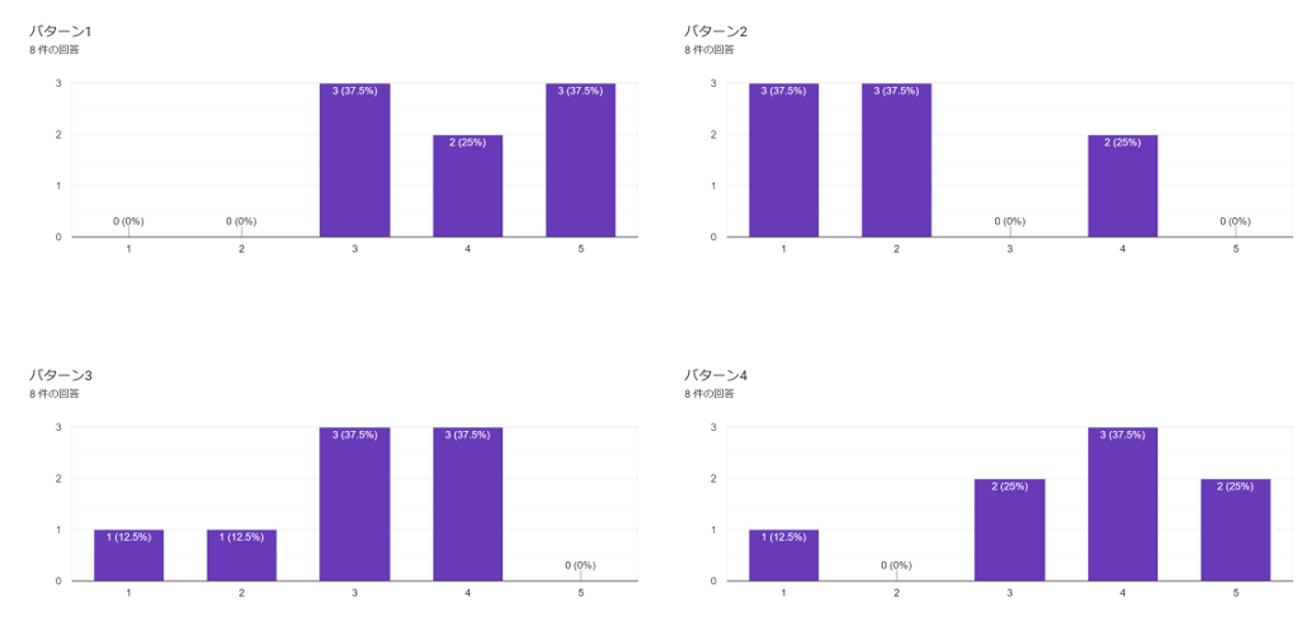
\includegraphics[clip,width=10cm]{./fig/incenerationAnk.png}
  \caption{アンケート結果(inceneration)}\label{inceAnk}
  \end{figure}
  


平均値を\ref{tab;inceAvera}に示す.これよりパターン1とパターン4の評価が高くなっている.
実験前アンケートと比較すると,実験者のイメージと同じ振動刺激を与えると没入感を高められることが分かる.
\begin{table}[h]
    \caption{平均値(inceneration)}
    \centering
    \begin{tabular}{l|l}
    \hline
    \hline
    パターン1 & 4\\
    パターン2 & 2.125\\
    パターン3 & 3\\
    パターン4 & 3.625\\
    \hline
    \end{tabular}
    \label{tab;inceAvera}
\end{table}

\newpage

\figref{ringAnk}にring-fire体験後のアンケートを示す.

\begin{figure}[h]
  \centering
  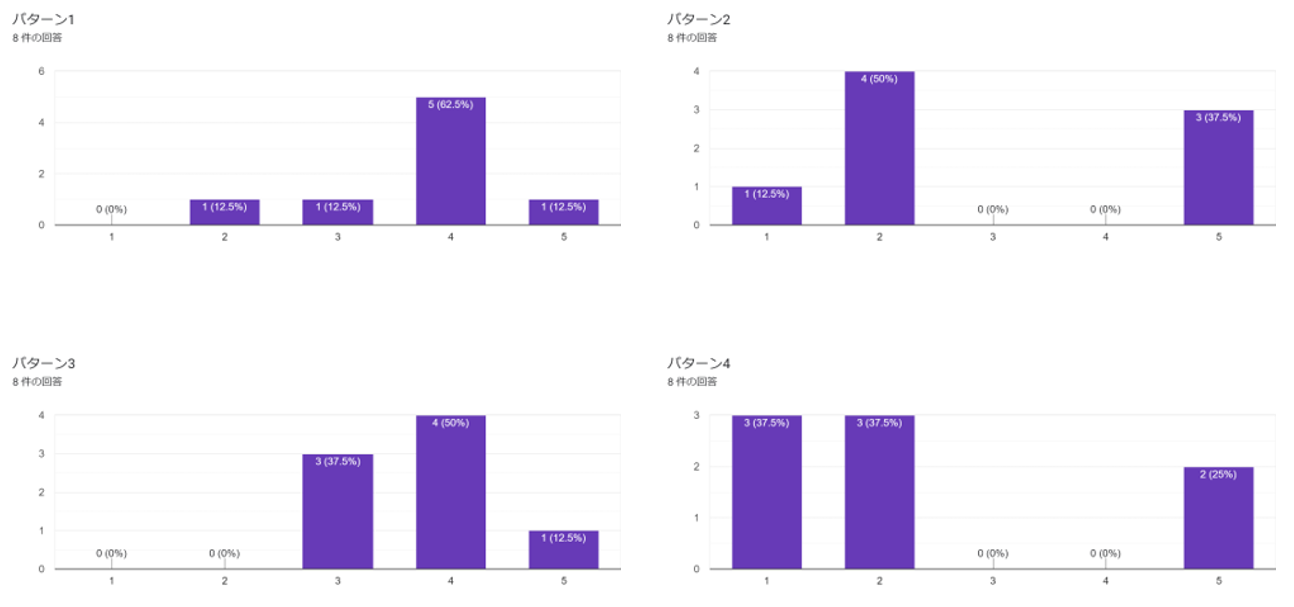
\includegraphics[clip,width=10cm]{fig/ringfireAnk.png}
  \caption{アンケート結果(ring-fire)}\label{ringAnk}
  \end{figure}


平均値を\ref{tab;ringAve}に示す.
パターン2の平均値が3.875と高くなっている.これは後から爆発が起こるという実験前アンケートの結果と一致していると言える.

\begin{table}[H]
    \caption{平均値(ring-fire)}
    \centering
    \begin{tabular}{l|l}
    \hline
    \hline
    パターン1 & 3.75\\
    パターン2 & 3\\
    パターン3 & 3.75\\
    パターン4 & 2.375\\
    \hline
    \end{tabular}
    \label{tab;ringAve}
\end{table}

\newpage
/figref{mainAnk}にmain-beam体験後のアンケート結果を示す.

\begin{figure}[h]
  \centering
  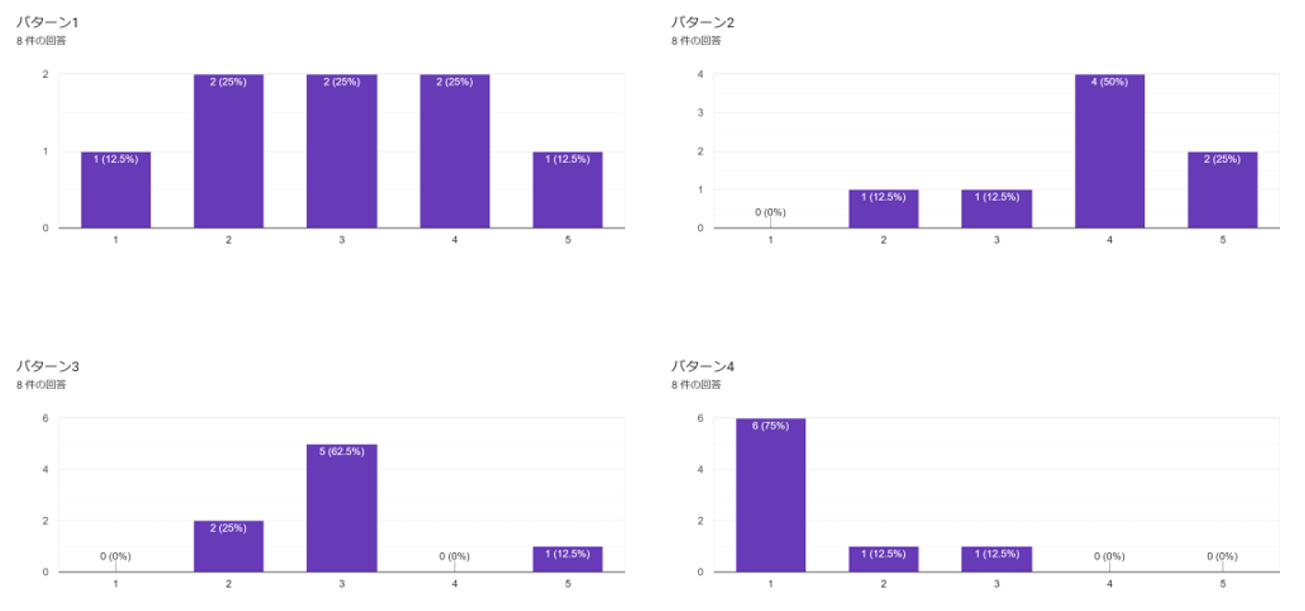
\includegraphics[clip,width=10cm]{fig/mainbeamAnk.png}
  \caption{アンケート結果(main-beam)}\label{mainAnk}
  \end{figure}


平均値を\ref{tab;mainAve}に示す.
パターン1とパターン3の評価が高くなっている.実験前アンケートの初めに大きい振動が来てその後余韻が残るという結果に沿っている.

  \begin{table}[H]
    \caption{平均値(main-beam)}
    \centering
    \begin{tabular}{l|l}
    \hline
    \hline
    パターン1 & 3\\
    パターン2 & 3.875\\
    パターン3 & 3\\
    パターン4 & 1.375\\
    \hline
    \end{tabular}
    \label{tab;mainAve}
\end{table}

事前アンケートの結果と同じような波形の振動パターンの評価が高くなる傾向にあった.

視覚エフェクトが大きくなるタイミングで振動も大きくなると視覚エフェクトと振動刺激が一致していると感じる傾向にある.


  % 第5章
\chapter{結論}




%%%%%%%%%%%%%%%%%%%%%%%%%%%%%%%%%%%%%%%%%%%%%%%%%%%%%%%%%%%%%%%%%%%%%%%
\begin{comment}
    \textblockcolour{pink}
    \begin{textblock}{4}(16, 1)
        【5】本文はここまで
    \end{textblock}
    
    \begin{textblock}{7}(11, 28)
        本文は20ページ以上を目安とする。
    \end{textblock}
\end{comment}
%%%%%%%%%%%%%%%%%%%%%%%%%%%%%%%%%%%%%%%%%%%%%%%%%%%%%%%%%%%%%%%%%%%%%%%
    % 第6章
% 謝辞
\theacknowledgments

本研究を進めるにあたり 井上 准教授,野田先生をはじめとした皆様からご指導,ご意見を頂きましたことに心より御礼申し上げます.

そして,レジュメや卒業論文を書く際に,ご指導頂きました島谷先輩,荒川先輩に御礼申し上げます.

最後になりましたが,日常の議論を通じて多くの知識や示唆を頂いた井上研究室の皆様に御礼申し上げます.ありがとうございました.
         % 謝辞
% 参考文献
\bibliographystyle{junsrt}      % bibTexのスタイル
\bibliography{./mybib}            % bibの読み込み


%%%%%%%%%%%%%%%%%%%%%%%%%%%%%%%%%%%%%%%%%%%%%%%%%%%%%%%%%%%%%%%%%%%%%%%

% \begin{comment}
%     \begin{textblock}{10}(7, 6)
%       本文中で参照をした文献だけを載せる
    
%       (本文中で参照していない文献を載せない)
%     \end{textblock}
    
%     \begin{textblock}{8}(11, 9.1)
%       ←Webページはアクセス日時を記載する
%     \end{textblock}
% \end{comment}
%%%%%%%%%%%%%%%%%%%%%%%%%%%%%%%%%%%%%%%%%%%%%%%%%%%%%%%%%%%%%%%%%%%%%%%

% 英語と日本語の参考文献が混在することを考慮してbiblatexは利用しない
% \printbibliography% 参考文献

%\input{appendix}   % 付録
\end{document}
